\documentclass{cshonours}
\usepackage{mathtools}
\usepackage{graphicx}
\usepackage{caption}
\usepackage{bm}
\usepackage[toc,page]{appendix}
\usepackage{listings}
\usepackage{courier}
\usepackage{url}
\usepackage{subfigure}
\usepackage{gensymb}
\usepackage{hyperref}
\usepackage{environ}
\usepackage{algorithm}% http://ctan.org/pkg/algorithms
\usepackage{algorithmicx}
\usepackage{algpseudocode}% http://ctan.org/pkg/algorithmicx
\usepackage{adjustbox}
\usepackage[table]{xcolor}
\usepackage{pdflscape}
\usepackage{multido}

\title{Faster Folding with kekrna \\ \normalsize Can't Spook the Zuke}
\author{Eliot Courtney \\ Student \#21141563}
\keywords{ribonucleic acid, dynamic programming, secondary structure, prediction}
\categories{J.3 Biology and genetics}

\date{\today}

\DeclarePairedDelimiter{\br}{\{}{\}}
\DeclarePairedDelimiter{\p}{(}{)}
\DeclarePairedDelimiter{\s}{[}{]}
\DeclarePairedDelimiter{\bo}{O(}{)}

\newcommand{\lyngso}{Lyngs{\o} }
\newcommand{\pushcode}[1]{\multido{\i=0+1}{#1}{\hskip\algorithmicindent}}

\newcommand{\AND}{\wedge}
\newcommand{\OR}{\vee}
\newcommand{\NOT}{\neg}
\newcommand{\IMPLIES}{\rightarrow}
\newcommand{\IFF}{\leftrightarrow}
\def\etal{et al. }
\def\km{kcal/mol }

\definecolor{verylightgray}{gray}{0.9}

\newcommand{\algautorefname}{Algorithm}
\newcommand{\algorithmautorefname}{Algorithm}
\newcommand{\chapautorefname}{Chapter}
\renewcommand{\chapterautorefname}{Chapter}
\renewcommand{\subsectionautorefname}{Subsection}
\renewcommand{\sectionautorefname}{Section}
\newcommand{\lineautorefname}{line}

\lstset{basicstyle=\ttfamily\footnotesize,breaklines=true}

\begin{document}
\maketitle
\begin{abstract}
I describe \emph{kekrna}, a new, fast ribonucleic acid folding package. Kekrna extends existing sparsification techniques to the Turner 2004 energy model including coaxial stacking, terminal mismatches, and dangles. In my benchmarks, kekrna is faster for minimum free energy folding and suboptimal structure generation than the current fastest package, ViennaRNA, even when ViennaRNA is given options disabling coaxial stacking. Kekrna is available at \url{https://github.com/Edgeworth/kekrna}.
\end{abstract}

\pagebreak
\vspace*{8cm}
\begin{center}
Copyright Eliot Courtney, 2016.
\end{center}

\begin{acknowledgements}
I would like to thank Max-Ward Graham and Professor Amitava Datta for their invaluable help and advice. I would also like to thank Andrew Gozzard for their help.
\end{acknowledgements}

\tableofcontents
\listoftables
\listoffigures
\allowdisplaybreaks

\chapter{Introduction and Background}
This dissertation is laid out in seven chapters. The first is this introduction, where I introduce the problem and explain what ribonucleic acid (henceforth RNA) and computational RNA folding is. The second talks about the energy model in detail, which is necessary for the discussion of the optimisations I applied to the Zuker-Stiegler algorithm. The third chapter describes the Zuker-Stiegler algorithm for free energy minimisation \cite{zukerDp} and the suboptimal folding algorithm of Wuchty et al \cite{wuchtySuboptimal}. The fourth chapter goes over a few of the existing implementations of the aforementioned algorithms. The fifth describes the main contribution of this dissertation: \emph{kekrna}, my RNA folding package. Kekrna uses and extends existing sparse folding techniques \cite{backofenSparseFolding, wexlerSparseFolding, willSparseFolding} to coaxial stacking, and also invents new sparsification techniques for suboptimal folding. In that chapter, I also describe other, less important algorithmic and implementation optimisations I did. The sixth chapter contains my benchmarking and accuracy results, in comparison to most of the currently popular RNA packages, and a discussion of those results. In the seventh and last chapter, I conclude with some discussion.

RNA (ribonucleic acid) is somewhat similar to DNA, but it is single stranded, and one of the four \emph{bases}, uracil, is different to that of DNA's, thymine. RNA is composed of a backbone of sugars, and the bases, which are just molecules, are attached to those sugars. We write down an RNA's \emph{primary structure} as a list of the four bases, guanine (G), uracil (U), adenine (A), and cytosine (C), which are often abbreviated to just the first letters. RNAs also have a direction, which we say goes from $5'$ to $3'$ (pronounced five-prime to three-prime). Each position on each sugar is given an identifier starting from $1'$; bases are connected at the $1'$ position, and phosphate groups on the $3'$ (to the next sugar) and $5'$ positions, forming the backbone of the RNA \cite{basicInfo}. Just like in DNA, these bases have other bases that they bind to. In RNA, these bonds happen between guanine and uracil (GU), guanine and cytosine (GC), and adenine and uracil (AU)---different to the only two canonical pairs that form in DNA: GC and AT. Because RNA is single-stranded, when the bases bind, they can bind to the RNA itself. This makes the RNA \emph{fold} and assume a shape.  Knowing the shape of RNA is useful for biologists to predict its function \cite{connRnaBackground}.

We separate the structure of RNA into three categories: primary structure, secondary structure, and tertiary structure. Primary structure is just the list of bases that make up the RNA. Secondary structure is how those bases bind to each other. Tertiary structure is the three-dimensional structure. To be more formal, we define the secondary structure of an RNA sequence $s \in \br{G, U, A, C}^*$ to be a set $S$ of base pairs $(st, en)$, $1 \leq st < en \leq |s|$, where $|s|$ is the length of the sequence, subject to a few constraints. Bases can only pair with one other base, so we require that $\forall (st, en), (st', en') \in S, st = st' \IFF en = en'$. It is also very common to disallow something called a pseudoknot, which is any two base pairs that overlap each other. Formally, a pseudoknot is two base pairings, $(st, en)$ and $(st', en')$ such that $st < st' < en < en'$. Without pseudoknots, all the base pairs form nested structures that are easily decomposable---in fact, \lyngso proved that the general RNA structure prediction problem, including pseudoknots, is NP-complete through a reduction from 3-SAT \cite{lyngsoPseudoknot}. When I talk about secondary structure, assume that it is secondary structure without pseudoknots.

There are three main methods of determining RNA structure. The first is physical experiments, like X-ray crystallography and nuclear magnetic resonance (NMR). People also use optical melting to determine the free energy of bonds. These physical experiments are time-consuming and expensive. The second is comparative sequence analysis, which is quite good but relies on lots of manual effort, expertise, and having a large number of similar sequences. It is considered the standard for evaluating the accuracy of the third type of prediction method: \emph{de novo} structure prediction \cite{tPartition}---which is almost always the only practical option. This refers to trying to predict the secondary or tertiary structure of an RNA from just its primary structure. This prediction method is what I will focus on for the rest of this review.

The major approach to predicting RNA structure is via free energy minimisation. Free energy is a measure of how much energy is available to do work in a system \cite{perrotThermodynamics}. The thermodynamic hypothesis \cite{anfinsenThermodynamicHypothesis} tells us to assume the structure RNA will assume \emph{in vivo} (in real life conditions) will have \emph{minimum free energy} (MFE)---this is also supported by evidence \cite{tinocoHowRnaFolds}. To compute the free energy, we need a model telling us how---I will go into detail about the current and historical models in the next section. Using that model, we can try to find the secondary structure which minimises the free energy. Usually, this is done through some form of dynamic programming---the Zuker-Stiegler algorithm---but there has also been some research into representing the folding problem as a stochastic context-free grammar, for example in CONTRAfold \cite{doContrafold}.

Kekrna implements the aforementioned Zuker-Stiegler algorithm with coaxial stacking, with some assumptions about the energy model. It assumes a Turner 04-like energy model, and is not as flexible as packages like RNAstructure \cite{rnastructure} and ViennaRNA \cite{viennarna} as to what energy models can be specified---in particular, the unpaired base cost is not configurable from the Turner 04 model value of zero. These are not inherent limitations---kekrna could be modified to support a similar set of data table parameters with no change in speed, except for the unpaired base cost, which, if positive, would impact performance somewhat.

\chapter{Energy Models}
\label{chap:energy}
An energy model, in the context of computational RNA folding, is something that tells us how to compute the free energy of some secondary structure. There are a few energy models that have been used in computational RNA folding, and all of the ones used in practice are a type of model called a \emph{nearest-neighbour} model. A nearest-neighbour model allows interactions between adjacent base pairs, and types of local substructures called loops. The types of loops in use in current energy models are explained below. Formally, Zuker and Sankoff define a loop, closed by a base pair $(ost, oen)$, to be the set of \emph{accessible} bases from $(ost, oen)$. A base $k$ is accessible from $(ost, oen)$ if, for all other base pairs $(ist, ien)$, it is not the case that $ost < ist < k < ien < oen$ \cite{zukerSankoff}. That is, there are not any base pairs ``between" $(ost, oen)$ and $k$. There could be accessible bases from $(ost, oen)$ that are in base pairs---those base pairs are called interior base pairs to the closing base pair $(ost, oen)$. The names $ost$, $oen$, $ist$, and $ien$ stand for ``outer start", ``outer end", ``inner start", and ``inner end" respectively. As an aside, the origin of the term \emph{nearest-neighbour model} seems murky---it certainly seems not to have originated in computational RNA folding.

The most used models are the so-called Turner 1999 \cite{t99} and Turner 2004 \cite{t04} models, compiled from various experiments. These models are similar, but Turner 2004 contains updated parameters that produce more accurate foldings, including a new model for multi-loops. There were models before these by Tinoco \cite{tinocoImprovedModel} and Salser \cite{salser}. Andronescu \etal produced a re-parametrisation of Turner 1999 through constrained optimisation, giving greater accuracy \cite{andronescuModel} and Aalberts and Nandagopal came up with a somewhat more different model \cite{aalbertsModel}. Kekrna implements the Turner 2004 energy model, which is the one used in RNAstructure \cite{rnastructure}.

I will now describe the different types of structures used to compute the free energy of a secondary structure. I will also introduce some notation that will be used throughout the rest of this dissertation---the \emph{dot-bracket} notation. Since we have assumed there are no pseudoknots, we can write the base pairs of an RNA using nested parentheses. Two bases are in a base pair if their parentheses match, and not bonded if they have a dot instead. For example, in the primary structure ``GAAAC", the dot-bracket string ``(...)" indicates that the G and C bases are paired, and the rest are not. We can then write the full secondary structure like this:

\begin{align*}
\texttt{GAAAC} \\
\texttt{(...)}
\end{align*}

This notation is useful for visualising the structure of loops when thinking about the dynamic programming algorithm. In this dissertation, I will also use angle brackets (\texttt{<   >}) to represent any substructure---i.e. any valid sequence of parentheses and dots. For a slightly more physical visualisation, something like what is shown in \autoref{fig:loop_structures} could be more useful. 

\begin{figure}[H]
\center
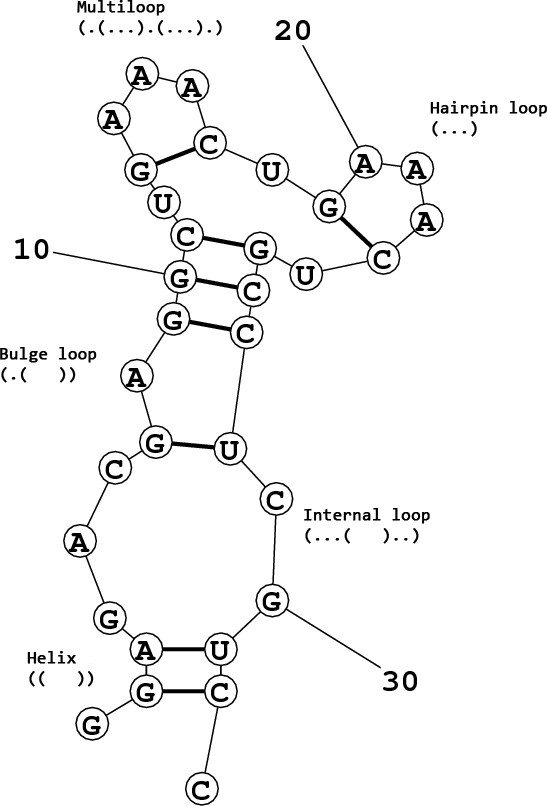
\includegraphics[width=0.7\textwidth]{res/model.png}
\caption{Different types of structures --- Generated using RNAstructure \cite{rnastructure}}
\label{fig:loop_structures}
\end{figure}

\subsection{Helices or ``Stacking"}
Helices are contiguous lengths of base pairs. To couch it in the definition of loop we provided, they are loops with exactly one interior base pair, $(ist, ien)$ to the exterior base pair $(ost, oen)$, and no unpaired bases. That is, $ist = ost + 1$ and $ien = oen - 1$ \cite{zukerSankoff}. These are energetically favourable because of what are called stacking interactions---$\pi$-bonds between the adjacent base pairs that stabilise the structure. In the Turner 1999 and 2004 models, these helices are assigned stabilising energies based on which base pairs are adjacent. For example, if an AU pair is followed by a GC pair, it is assigned a free energy of -2.08 kcal/mol. There is also a case where one special sequence of four base pairs is given a different free energy, but as far as I can tell this is not implemented by any RNA folding packages, including kekrna, although it would not be very hard to add.

Whenever a helix is ended or started by a base pair that is AU, GU, UG, or UA, a special \emph{AU/GU penalty} is applied. In the case of a length one helix it is still applied twice---once when it starts and once when it ends. The name ``stacking" is a bit confusing, because there is also \emph{coaxial stacking}, which is different. Whenever I am talking about coaxial stacking, I will always prefix the word ``coaxial".

In dot-bracket notation, helices are shown as concentric parentheses, like this:
$$\texttt{((((<...>))))}$$

\begin{algorithm}[H]
\caption{Computes the energy of a helix where $r$ is a primary sequence, with $(ost, oen)$ as an outer base pair, and $(ist, ien)$ as an inner base pair}
\label{alg:stacking_energy}
\begin{algorithmic}
\Function{StackingEnergy}{$r, ost, oen, ist, ien$}
\State $e \gets$ the stacking value you look up in a table
\State \Return $e$
\EndFunction
\end{algorithmic}
\end{algorithm}

\subsection{Hairpin Loops}
Having helices necessarily means that sometimes we must form loops. These are generally energetically unfavourable. A hairpin loop is a sequence of at least three unpaired bases closed by a base pair---that is, it is a loop with no interior base pairs. There has been a lot of research done on hairpin loops, and there are many special interactions that have been observed. For example, there are special tetraloops (a hairpin loop with four unpaired bases in it) that have their own recorded energy values in the Turner 2004 and Turner 1999 models \cite{t99, t04}. The technical details of the hairpin loop energy function will be relevant later, so I present here the algorithm for computing the energy. I am using substring notation like Python's, except that slices use inclusive indices. It is zero-based and you can also look up negative indices: $r[-k] = r[|r| + k]$. Here, and for the rest of the dissertation, $r$ refers to the primary sequence. You can use a slice notation to get a substring: $r[a:b] = r[a] + r[a + 1] + \cdots + r[b]$. So $r[1:-1]$ means ``take the substring starting at index 1 and going all the way to the end." If you see a constant that has not been defined anywhere (like ``GGFirstMismatch"), then it is a parameter of the energy model, and the value can be found in the Nearest Neighbour Database (NNDB) \cite{tNndb}.


In dot-bracket notation, hairpin loops look like one pair of parentheses, with at least three dots in the middle:
$$\texttt{(...)}$$

\begin{algorithm}[H]
\caption{Computes the energy of a hairpin loop, where $r$ is a primary sequence, $r[st:en]$ is the hairpin loop, and $(r[st], r[en])$ is the closing base pair.}
\label{alg:hairpin_energy}
\begin{algorithmic}
\Function{HairpinEnergy}{$r$, $st$, $en$}
\If{$r[st:en] \in$ SpecialHairpins}
\State \Return SpecialHairpins[$r[st:en]$]
\EndIf
\State $length \gets en - st - 1$
\State $e \gets InitiationEnergy[length]$ \Comment{Defined by a formula \cite{tNndb}}
\If{$(r[st], r[en])$ is AU/GU in any order}
\State $e \gets e + AuGuPenalty$
\EndIf
\If{$length = 3$}\Comment{Separate rules for size 3 hairpins}
\If{$r[st+1:en-1]$ are all C bases}
\State $e \gets e + AllC.three$ \Comment{All-C value for size 3 hairpins}
\EndIf
\Else
\State $e \gets e + TerminalMismatchEnergy(r[st], r[st + 1], r[en-1], r[en])$
\If{$(r[st+1], r[en-1])$ is exactly UU or GA}
\State $e \gets e + UUGAFirstMismatch$
\ElsIf{$(r[st+1], r[en-1])$ is GG}
\State $e \gets e + GGFirstMismatch$
\EndIf
\If{$r[st+1:en-1]$ are all C bases}
\State $e \gets e + AllC.a \times length + AllC.b$
\EndIf
\If{$(r[st], r[en])$ is exactly GU \bf{and} \\
\pushcode{3} $st \geq 2$ \bf{and} $r[st - 1] = r[st - 2] = G$}
\State $e \gets e + SpecialGuClosure$
\EndIf
\EndIf
\State \Return e
\EndFunction
\end{algorithmic}
\end{algorithm}

\subsection{Bulge Loops}
Bulge loops are loops that have exactly one interior base pair, $(ist, ien)$, and have no unpaired bases on one side of the exterior (closing) base pair, $(ost, oen)$. That is, exactly one of $ist = ost + 1$ or $ien = oen - 1$ is true. This is because the ``bulging" unpaired base is pushed out and the stacking interactions can continue as if it were not there between the otherwise adjacent base pairs. Like hairpin loops, Turner 2004 defines a complicated piecewise function that depends on how many unpaired bases there are and what kind of bases are inside the bulge loop \cite{tNndb}.

\begin{algorithm}[H]
\caption{Computes the energy of a bulge loop, where $r$ is a primary sequence, $(ost, oen)$ is the outer base pair, and $(ist, ien)$ is the inner base pair.}
\label{alg:bulge_energy}
\begin{algorithmic}
\Function{BulgeEnergy}{$r, ost, oen, ist, ien$}
\State $length \gets \max(ist - ost, oen - ien) - 1$
\State $e \gets BulgeInitiation[length]$ \Comment{Defined by a formula \cite{tNndb}}
\If{$length > 1$} \Comment{These treated as separate helices}
\If{$(r[ost], r[oen])$ is AU/GU in any order}
\State $e \gets e + AuGuPenalty$
\EndIf
\If{($r[ist], r[ien])$ is AU/GU in any order}
\State $e \gets e + AuGuPenalty$
\EndIf
\State \Return $e$
\EndIf
\State $e \gets e + StackingEnergy(r[ost], r[ist], r[ien], r[oen])$
\State $unpaired \gets$ the index of the single unpaired base in the bulge
\If{$r[unpaired] = C$ \textbf{and} \\
\pushcode{3} ($r[unpaired - 1] = C$ \textbf{or} $r[unpaired + 1] = C$)}
\State $e \gets e + SpecialCBulge$
\EndIf
\State $states \gets$ the number of contiguous equal bases including $r[unpaired]$
\State $e \gets 10 \times R \times T \log states$
\State \Return $e$
\EndFunction
\end{algorithmic}
\end{algorithm}

In dot-bracket notation, bulge loops have two parentheses adjacent to each other on one side, and at least one unpaired base between the two parentheses on the other side:
$$\texttt{((<...>)..)}$$

\subsection{Internal Loops}
Internal loops look like bulge loops, but they also have one or more unpaired bases on the other side. Formally, $ist > ost + 1$ and $ien < oen - 1$. These are often lumped together with bulge loops and stacking, as they can be generalised to something sometimes referred to as a \emph{two-loop} \cite{zukerSankoff}, since the only difference between them is that internal loops have unpaired bases on both sides. There are, again, special cases for internal loops up to size two by three (two unpaired bases on one side, three unpaired bases on the other). \autoref{alg:internal_energy} shows the algorithm for internal loops, and \autoref{alg:twoloop_energy} shows the combined algorithm for two-loops.

In dot-bracket notation, internal loops look like bulge loops, except they must have at least one unpaired base between the two parentheses on both sides:
$$\texttt{(...(<...>)..)}$$

\begin{algorithm}[H]
\caption{Computes the energy of an internal loop, where $r$ is a primary sequence, $(ost, oen)$ is the outer base pair, and $(ist, ien)$ is the inner base pair.}
\label{alg:internal_energy}
\begin{algorithmic}
\Function{InternalEnergy}{$r, ost, oen, ist, ien$}
\If{this is a special internal loop}
\State \Return $SpecialInternalLoop(r, ost, oen, ist, ien)$
\EndIf
\State $toplength \gets ist - ost - 1$
\State $botlength \gets oen - ien - 1$
\State $e \gets InternalInitiation[toplength + botlength]$
\If{$(r[ost], r[oen])$ is AU/GU in any order}
\State $e \gets e + InternalAuGuPenalty$
\EndIf
\If{$(r[ist], r[ien])$ is AU/GU in any order}
\State $e \gets e + InternalAuGuPenalty$
\EndIf
\State $asym \gets \min(|toplen-botlen| \times InternalAsym, NinioMaxAsym)$ \footnotemark
\State $e \gets e + asym$
\If{this internal loop is 2x3 or 3x2}
\State $e \gets e + Internal2x3Mismatch(r[ost], r[ost+1], r[oen-1], r[oen])$
\State $e \gets e + Internal2x3Mismatch(r[ien], r[ien+1], r[ist-1], r[ist])$
\Else
\State $e \gets e + InternalOtherMismatch(r[ost], r[ost+1], r[oen-1], r[oen])$
\State $e \gets e + InternalOtherMismatch(r[ien], r[ien+1], r[ist-1], r[ist])$
\EndIf
\State \Return $e$
\EndFunction
\end{algorithmic}
\end{algorithm}

\footnotetext{This Ninio maximum asymmetry term is not documented in the NNDB anywhere, but it is implemented by RNAstructure, and is alluded to by \lyngso \cite{lyngsoOptimisation}}

\begin{algorithm}[H]
\caption{Computes the energy of either an internal loop, a bulge loop, or stacking. }
\label{alg:twoloop_energy}
\begin{algorithmic}
\Function{TwoLoopEnergy}{$r, ost, oen, ist, ien$}
\State $toplength \gets ist - ost - 1$
\State $botlength \gets oen - ien - 1$
\If{$toplength = 0$ \bf{and} $botlength = 0$}
\State \Return \Call{StackingEnergy}{$r, ost, oen, ist, ien$}
\ElsIf{$toplength \geq 1$ \bf{and} $botlength \geq 1$}
\State \Return \Call{InternalEnergy}{$r, ost, oen, ist, ien$}
\Else
\State \Return \Call{BulgeEnergy}{$r, ost, oen, ist, ien$}
\EndIf
\EndFunction
\end{algorithmic}
\end{algorithm}

\subsection{Multi-loops}
Multi-loops are loops with multiple interior base pairs. The areas closed by the base pairs in a multi-loop are called branches, including the closing (or outer) base pair. There are some additional interactions that have been added since the original Zuker-Stiegler algorithm, such as \emph{coaxial stacking}, which is where adjacent branches can have stacking interactions between their closing base pairs. These will be explained in the next section.

Multi-loops are poorly predicted by the Turner models. Even though the Turner 1999 and 2004 models give logarithmic and asymmetry based equations describing the free energy of multi-loops, in practice, these are not used for free energy minimisation---instead, an affine approximation is used \cite{sankoffKruskal, mainville}. Until recently, there was no known polynomial algorithm that computed the MFE structure in a logarithmic or asymmetry-based model. Ward, Datta, and Mathews have come up with an $O(N^4)$ time algorithm that is applicable to logarithmic, and even more general energy models \cite{wardPersonal}.

Kekrna uses the same affine approximation as RNAstructure, which is where:
\begin{align*}
BranchCost &= -0.6 \km \\
Initiation &= 9.3 \km \\
\end{align*}

But, there is another setting commonly used, where $BranchCost = -0.9 \km$ \cite{t04}. 

In dot-bracket notation, a multi-loop looks like an outer pair with at least two branches inside, separated by any number of unpaired bases:
$$\texttt{(..(<...>)(<...>).)}$$

Note that \autoref{alg:multiloop_energy}, like \autoref{alg:internal_energy} et. cetera, only computes the energy contribution from the loop itself, not the structures it contains.

\begin{algorithm}[H]
\caption{Computes the energy of a multi-loop.}
\label{alg:multiloop_energy}
\begin{algorithmic}
\Function{MultiloopEnergy}{$NumBranches$}
\State \Return $NumBranches \times BranchCost + Initiation$
\EndFunction
\end{algorithmic}
\end{algorithm}


\subsection{Coaxial Stacking, Dangling Ends, and Terminal Mismatches}
\emph{Coaxial stacking} is a stacking interaction between the closing base pairs of adjacent branches, or branches separated by one unpaired base, and has been shown to increase the accuracy of RNA secondary structure prediction \cite{tNndb, walterCoaxial}. Coaxial stacking is a relatively recent development, and still most of the contemporary RNA folding packages do not handle it well. Coaxial stacking is one of the three possible interactions that can occur with branches in the Turner 2004 model, the other two being dangling ends and terminal mismatches. A \emph{dangling end} is the interaction of an unpaired base adjacent to a branch. There are two types, $3'$ and $5'$, depending on which side of the branch it is on---if it is on the $5'$ side of the branch, it is called a $5'$ dangle. If a branch has an unpaired base adjacent on both sides, they cannot both dangle. Instead, they can form what is called a \emph{terminal mismatch}, which is counted differently in the energy model. A branch or unpaired base can only be involved in at most one of these three interactions, and to compute the MFE structure, we need to take the combination of interactions that gives the lowest free energy. This significantly complicates the Zuker-Stiegler prediction algorithm (to be explained in the next section), and is likely part of the reason that RNA folding including these interactions is poorly implemented by many RNA packages.

There are two types of coaxial stacking: flush coaxial stacking, and mismatch-mediated coaxial stacking. In flush coaxial stacking, two branches directly adjacent to each other stack on top of each other in an energetically favourable way. It looks like this in dot-bracket notation: \texttt{(...)(...)}. Mismatch-mediated coaxial stacking is similar, but has an unpaired base in-between the branches: \texttt{L(...).(...)R}, and is counted differently in the energy model. The unpaired base can form a terminal mismatch with either L or R in the previous example. The energy is determined by looking up a value based on the two bases in the terminal mismatch, and the two bases in the base pair of the branch straddled by the terminal mismatch.

I break down flush coaxial stacking into two types: \emph{normal}, and \emph{outer}. The normal type looks like the previous example. The outer type happens when one of the branches is the outer loop in a multi-loop, and looks like this: \texttt{((.A.).<   >..)}. Here, the branch indicated by A is in an outer flush coaxial stack with the outer (or \emph{closing}) branch. I also break down mismatch mediated coaxial stacking into six types: \emph{left}, \emph{right}, \emph{left outer}, \emph{right outer}, \emph{left inner}, and \emph{right inner}. The first two do not involve an outer loop, the rest do. I summarise what they look like in \autoref{table:coax_types}.

\rowcolors{1}{white}{verylightgray}
\begin{table}
\begin{adjustbox}{center}
\begin{tabular}{ll}
left & \texttt{.(...).(...)} \\
right & \texttt{(...).(...).} \\
left outer & \texttt{(.(...)<   >.)} \\
right outer & \texttt{(.<   >(...).)} \\
left inner & \texttt{(.(...).<   >)} \\
right inner & \texttt{(<   >.(...).)} \\
\end{tabular}
\end{adjustbox}
\caption{Types of coaxial stacks}
\label{table:coax_types}
\end{table}
\rowcolors{1}{white}{white}

So that kekrna can report the combination of coaxial stacking, dangling ends, and terminal mismatches (henceforth referred to as \emph{CTDs}), I invented an extension to the dot-bracket notation which also includes CTD information. Parentheses are replaced by square brackets (to differentiate between a secondary structure with no CTDs and one with none specified). Dangles are represented by ``5" and ``3" for $5'$ and $3'$ dangles respectively. Terminal mismatches are represented by ``m" and ``M", for the unpaired bases that are on the $5'$ side and $3'$ side, respectively. It is necessary to use two different symbols here, rather than lower-case ``m" for both, as there would otherwise be ambiguous cases. The Turner 04 model allows branches to be in two coaxial stacks: one as an internal branch to a multi-loop, and another as the outer branch of a multi-loop. In the following example, branches are indicated by the letter they contain, except for the outer branch of the multi-loop on the right, which is B. The branch B can be involved in a flush coaxial stack with both A, and C or D. 

$$\texttt{(.A.)((.C.)(.D.))}$$

To be able to store both of these interactions, I put the interaction of the branch as an internal branch in the location where the left square bracket would be, and the interaction of the branch as the outer branch of a multi-loop where the right square bracket would be. A branch in a coaxial stack can either interact with the previous branch (in the $5'$ direction), or the next branch (in the $3'$ direction), which I encode as ``p" for previous, and ``n" for next. In the case of an outer branch, these are capitalised, and next refers to the first internal branch in that multi-loop.

In the example shown in \autoref{fig:ctd_notation}, the first line indicates the names I am giving to the branches below, which are in normal dot-bracket notation. The last line shows the CTD interactions. Branch A is involved in a terminal mismatch, and a $3'$ dangle. Branches B and C have no interactions. Branch D is in a flush coaxial stack with E. Branch F has a $5'$ dangle. Branch E additionally, as an outer loop, is involved in a flush coaxial stack with G.
\begin{figure}
\begin{align*}
\texttt{.A.B....C........D....E...F.....G.....} \\
\texttt{.(.(...)(...))...(...)(...(...).(...))} \\
\texttt{m[3[...][...]]M..n...]p..5[...].n...]P}
\end{align*}
\caption{CTD notation}
\label{fig:ctd_notation}
\end{figure}

\chapter{The Algorithms}
\section{The Zuker-Stiegler Algorithm Without CTDs}
The Zuker-Stiegler algorithm is an important dynamic programming algorithm in computational RNA folding, and what my project is mainly about. It computes the secondary structure of a primary structure with the minimum free energy in $\bo{N^3}$ time using $\bo{N^2}$ memory \cite{zukerDp}. It is the basis of the main RNA folding packages today. I will discuss those packages in \autoref{chap:work}.

Prior to the Zuker-Stiegler algorithm, there was work done by Nussinov \cite{nussinovDp} and Studnicka et al. \cite{studnickaDp}. The ideas from these works were used as a basis by Zuker and Stiegler \cite{zukerDp}. The Nussinov algorithm only tries to maximise the number of base pairs. The algorithm of Studnicka et al. is slow. The Zuker-Stiegler algorithm is an improvement over both of these because it incorporates a nearest-neighbour type energy model to minimise the free energy, and is relatively fast.

I will now describe a version of the Zuker-Stiegler algorithm. Note that all indices are inclusive, and it assumes that the unpaired base cost is zero, as is the case in the Turner 2004 model. First, we define some useful helper functions. Again, if there are undefined names like $AuGuPenalty$, they refer to constants of the energy model. The function $ViablePair(st, en)$ checks if $(st, en)$ can form a base pair and that they are not \emph{lonely pairs}. Lonely pairs (or isolated pairs) are pairs that do not have any neighbours (the potential pairs $(st + 1, en - 1)$ and $(st - 1, en + 1)$) that could possibly pair \cite{mathewsLonely}.

\begin{align*}
N &= \text{the size of the primary structure} \\
MinHairpinSize &= 3 \\
AuGu(st, en) &= \begin{dcases*}
AuGuPenalty & if the pair (st, en) is AU/GU \\
0 & otherwise \\
\end{dcases*} \\
ViablePair(st, en) &= \begin{dcases*}
\bf{true} & if (st, en) can pair and is not a lonely pair \\
\bf{false} & otherwise \\
\end{dcases*} \\
\end{align*}

Structures that are not inside any other structures (like a multi-loop) are said to be in the \emph{exterior loop}. This is mostly handled as if it were a multi-loop, but there is no initiation, branch, or unpaired base cost. The $Ext(st)$ function finds the energy of the best exterior loop that starts at or after $st$, via the observation that the base at $st$ is either paired or it is not.
\begin{align*}
Ext(N) &= 0 \\
Ext(st) &= \min \begin{dcases}
  Ext(st + 1) \\
  Pair \quad \forall en \ni st < en < N  \\
\end{dcases} \\
Pair &= Paired(st, en) + AuGu(st, en) + Ext(en + 1) \\
\end{align*}

The function $TwoLoop(st, en)$ finds the energy of the best two loop with the outer base pair $(st, en)$. It only considers loops up to size thirty, which is a standard hack to make the algorithm run in $O(N^3)$ time rather than $O(N^4)$ time. \lyngso came up with a method to find the best two-loop in $O(N^3)$ time, but also found that just checking up to length thirty was good enough most of the time \cite{lyngsoOptimisation}.
\begin{align*}
TwoLoop(st, en) &= \min_{\substack{st < ist < ien < en\\ 1 \leq ist - st - 1 + en - ien - 1 \leq 30}}{
  TwoLoopPair
} \\
TwoLoopPair &= TwoLoopEnergy(st, en, ist, ien) + Paired(ist, ien) \\
\end{align*}

The $Paired(st, en)$ function finds the energy of the best structure given that $st$ and $en$ are paired. A multi-loop must contain at least three branches: two internal branches and one outer branch. So, we need an extra function, $Unpaired2$, which tells us the energy of the best structure that has at least two (internal) branches. Paired could alternately be implemented by minimising $Unpaired(st, piv) + Unpaired(piv + 1, en)$ over all split points $piv$, but this would not be \emph{canonical}, which I will explain later. I have split the $Stacking$ case out separately in $Paired$, but it could be handled equally well as part of $TwoLoop$.
\begin{align*}
Paired(st, en) &= \infty \text{ when } \NOT ViablePair(st, en) \\
Paired(st, en) &= \min{\begin{dcases}
  Hairpin(st, en) \\
  Stacking \\
  TwoLoop(st, en) \\
  Multiloop \\
\end{dcases}} \\
Stacking &= StackingEnergy(st, en, st + 1, en - 1) + Paired(st + 1, en - 1) \\
Multiloop &= Unpaired2(st + 1, en - 1) + AuGu(st, en) \\
  &+ BranchCost + Initiation \\
\end{align*}

The $Unpaired(st, en)$ function finds the energy of the best structure with at least one branch, where $st$ and $en$ do not have to be paired. We assume we are inside a multi-loop in this function, so we have to add branch costs. This is why we need a separate function for the exterior loop.
\begin{align*} 
Unpaired(x, x) &= \infty \text{ --- Must contain at least one branch.} \\
Unpaired(st, en) &= \min{\begin{dcases*}
  Paired(st, en) + BranchCost & Try pairing at [st, en] \\
  Unpaired(st + 1, en) & Assume st is not paired. \\
  Pair \quad \forall piv \ni st < piv < en & Assume st is paired. \\
\end{dcases*}} \\
Pair &= Paired(st, piv) + AuGu(st, piv)  \\
  &+ BranchCost + min(Unpaired(piv + 1, en), 0) \\
\end{align*}

The previously mentioned $Unpaired2$ function finds the best structure with at least two branches, where $st$ and $en$ do not have to be paired. It is the same as $Unpaired$, except for the two branch requirement.
\begin{align*}
\text{}& \\
Unpaired2(x, x) &= \infty \text{ --- Must contain at least two branches.} \\
Unpaired2(st, en) &= \min{\begin{dcases*}
  Unpaired2(st + 1, en) & Assume st is not paired. \\
  Pair \quad \forall piv \ni st < piv < en & Assume st is paired. \\
\end{dcases*}} \\
Pair &= Paired(st, piv) + AuGu(st, piv)  \\
  &+ BranchCost + Unpaired(piv + 1, en) \\
MFE() &= Ext(0)
\end{align*}

Finally, we get the MFE from the value of $Ext(0)$, which is the energy of the best exterior loop starting at or after $0$. 

The basic Zuker-Stiegler algorithm can be formulated in many different ways. It is very important that the formulation is \emph{canonical}---that is, it should only consider a particular structure once. For example, you can compute $Unpaired(st, en)$ by dividing it into two calls to $Unpaired$, rather than one call to $Paired$ and one call to $Unpaired$. This gives the same answer for the MFE, but potentially considers the same structures more than once, since $Unpaired(st, piv)$ might have the same MFE structure as $Unpaired(st, piv + 1)$. If you do not have canonicality, then it is harder during suboptimal folding to not generate duplicate structures, which imposes a performance penalty. The formulation I just gave is canonical.

In real implementations, rather than as a series of mutually recursive functions, the Zuker-Stiegler algorithm is usually done as a bottom-up fill of dynamic programming tables. For each function, you make a table that stores the value of running that function for every possible input. Since every function above only has two arguments that go from $0$ to $N$, it uses $O(N^2)$ memory in tables. The functions looking at internal loops have them limited to size thirty, so that part is $O(1)$. But, some functions use $O(N)$ time looking at split points, the overall time complexity is $O(N^3)$.

To recover an MFE structure (there may be multiple), you start at $Ext(0)$, then look at each part of the recurrence to find where $Ext(0)$ came from---for example, $Ext(0)$ might have come from $Paired(0, 5)$ and $Ext(6)$. Recursively following these lets you reconstruct an MFE structure. This type of approach is discussed in more detail by Zuker and Sankoff \cite{zukerSankoff}.

\section{The Zuker-Stiegler Algorithm With CTDs}
\label{sec:zuker_ctd}
Adding CTDs to the Zuker-Stiegler algorithm significantly complicates it. I here present \emph{the kek manoeuvre}, which is the formulation of the Zuker-Stiegler algorithm with CTDs that I invented. It considers branches separately when finding the optimal CTD configuration, which is different to the other ways of doing it. One other way is to consider all possible CTD configurations of two branches in each range $(st, en)$ and store that in a table specifically for coaxial stacking. Using the kek manoeuvre turns out to be important for optimisation using sparse folding, which I discuss in \autoref{ssec:sparse}.

A lot of the basic ideas from the formulation without CTDs are the same. First, we need some more helper functions. The kek manoeuvre sometimes needs to infer what a paired base must be based on whether it is in a Watson-Crick or GU pair, when it cannot know what that base's index is. 
\begin{align*}
WC(b) &= \text{The Watson-Crick complement of } b \\
GU(b) &= \text{The GU complement of } b \\
StackingBaseEnergy &= \text{the same as } StackingEnergy \text{ but look up using bases} \\
\end{align*}

We start by again defining the function $Ext$.
\begin{align*}
Ext(N) &= 0 & \quad \triangleright \text{ Base case} \\
Ext(st) &= \min{\begin{dcases*}
  Ext(st + 1) & \\
  NoCTD \quad \forall en \ni st < en < N & \\
  Dangle3' \quad \forall en \ni st < en < N & \\
  Dangle5' \quad \forall en \ni st < en < N & \\
  Mismatch \quad \forall en \ni st < en < N & \\
  LeftCoaxWC \quad \forall en \ni st < en < N & \\
  LeftCoaxGU \quad \forall en \ni st < en < N &  \\
  RightCoaxFwd \quad \forall en \ni st < en < N & \\
  FlushCoaxWC \quad \forall en \ni st < en < N - 1 & \\
  FlushCoaxGU \quad \forall en \ni st < en < N - 1 & when $r[en + 1]$ is G or U \\
\end{dcases*}} \\
NoCTD &= Paired(st, en) + AuGu(st, en) \\
  &+ Ext(en + 1) \\
Dangle3' &= Paired(st, en - 1) + AuGu(st, en - 1) \\
  &+ Dangle3Energy(en - 1, en, st) + Ext(en + 1) \\
Dangle5' &= Paired(st + 1, en) + AuGu(st + 1, en) \\
  &+ Dangle5Energy(en, st, st + 1) + Ext(en + 1) \\
Mismatch &= Paired(st + 1, en - 1) + AuGu(st + 1, en - 1) \\
  &+ MismatchEnergy(en - 1, en, st, st + 1) + Ext(en + 1) \\
LeftCoaxWC &= Paired(st + 1, en - 1) + AuGu(st + 1, en - 1) \\
  &+ MismatchCoaxEnergy(en - 1, en, st, st + 1) + ExtWC(en + 1) \\
LeftCoaxGU &= Paired(st + 1, en - 1) + AuGu(st + 1, en - 1) \\
  &+ MismatchCoaxEnergy(en - 1, en, st, st + 1) + ExtGU(en + 1) \\
RightCoaxFwd &= Paired(st, en - 1) + AuGu(st, en - 1) \\
  &+ ExtRightCoax(en + 1) \\
FlushCoaxWC &= Paired(st, en) + AuGu(st, en) \\
  &+ StackingBaseEnergy(r[en], r[st], r[en + 1], WC(r[en + 1])) \\
  & + ExtWC(en + 1) \\
FlushCoaxGU &= Paired(st, en) + AuGu(st, en) \\
  &+ StackingBaseEnergy(r[en], r[st], r[en + 1], GU(r[en + 1])) \\
  &+ ExtGU(en + 1) \\
\end{align*}

It is similar to the $Ext$ of the basic formulation, but it has a lot of extra cases. It can be confusing to understand what each of these cases means. So, in \autoref{table:ext_cases} I list the corresponding dot-bracket structure for each case.

\rowcolors{1}{white}{verylightgray}
\begin{table}[h]
\begin{adjustbox}{center}
\begin{tabular}{ll}
NoCTD & \texttt{(...)<   >} \\
Dangle3' & \texttt{(...)3<   >} \\
Dangle5' & \texttt{5(...)<   >} \\
Mismatch & \texttt{.(...).<   >} \\
LeftCoaxWC & \texttt{.(...).<(...) >} \\
LeftCoaxGU & \texttt{.(...).<(...) >} \\
RightCoaxFwd & \texttt{(...).<(...). >} \\
FlushCoaxWC & \texttt{(...)<(...) >} \\
FlushCoaxGU & \texttt{(...)<(...) >} \\
\end{tabular}
\end{adjustbox}
\caption{Ext function cases}
\label{table:ext_cases}
\end{table}
\rowcolors{1}{white}{white}

For dealing with CTDs we need to add a few new functions: $ExtGU$, $ExtWC$, and $ExtRightCoax$. The $ExtGU(st)$ function returns the MFE given that $st$ is in a GU or UG pair. The function $ExtWC$ is similar, but for Watson-Crick pairs. Suppose we are trying to make a flush coaxial stack with the left branch at $(a, b)$. We know the right branch starts at $b + 1$ and what base that is. If we knew whether it was closed by a Watson-Crick or GU/UG pair, we would know what the final base is, and be able to work out the energy. This is what these two functions are for. Left mismatch coaxial stacks also work with this method, since we trivially know all the bases. Right mismatch coaxial stacks are tricky and require the $ExtRightCoax(st)$ function. It gives the MFE of the best structure given that a branch starts at $st$ and is involved backwards in a right coaxial stack. In the context of $ExtRightCoax(st)$ we trivially know all the bases required to compute the energy, so we do it there. These ideas of a $GU$, $WC$ and $RightCoax$ function are repeated in the $Unpaired$ and $Unpaired2$ functions.
\begin{align*}
ExtWC(N) &= \infty \\
ExtWC(st) &= \min{\begin{dcases*}
  Pair \quad \forall en \ni st < en < N & if $(st, en)$ is Watson-Crick \\
  \infty & otherwise \\
\end{dcases*}} \\
ExtGU(N) &= \infty \\
ExtGU(st) &= \min{\begin{dcases*}
  Pair \quad \forall en \ni st < en < N & if $(st, en)$ is GU/UG \\
  \infty & otherwise \\
\end{dcases*}} \\
Pair &= Paired(st, en) + AuGu(st, en) + Ext(en + 1) \\
ExtRightCoax(N) &= \infty \\
ExtRightCoax(st) &= \min{\begin{dcases*}
  RightCoaxBack \quad \forall en \ni st < en < N & if $st > 0$ \\
  \infty & otherwise \\
\end{dcases*}} \\
RightCoaxBack &= Paired(st, en - 1) + AuGu(st, en - 1) \\
  &+ MismatchCoaxEnergy(en - 1, en, st - 1, st) \\
  & + Ext(en + 1) \\
\end{align*}


The $Paired(st, en)$ function returns the energy of the best structure given $(st, en)$ is paired. There are many more cases we need to handle, but that is it.
\begin{align*}
Paired(st, en) &= \infty \text{ when } \NOT ViablePair(st, en) \\
Paired(st, en) &= \min{\begin{dcases*}
  Hairpin(st, en) \\
  Stacking \\
  TwoLoop(st, en) \\
  Multiloop \\
  OuterDangle3' \\
  OuterDangle5' \\
  OuterMismatch \\
  LeftOuterCoax \quad \forall piv \ni st < piv < en \\
  RightOuterCoax \quad \forall piv \ni st < piv < en \\
  LeftInnerCoax \quad \forall piv \ni st < piv < en \\
  RightInnerCoax \quad \forall piv \ni st < piv < en \\
  LeftFlushCoax \quad \forall piv \ni st < piv < en \\
  RightFlushCoax \quad \forall piv \ni st < piv < en \\
\end{dcases*}} \\
Stacking &= StackingEnergy(st, en, st + 1, en - 1) + Paired(st + 1, en - 1) \\
BaseCost &= AuGu(st, en) + BranchCost + Initiation \\
Multiloop &= BaseCost + Unpaired2(st + 1, en - 1) \\
OuterDangle3' &= BaseCost + Unpaired2(st + 2, en - 1) \\
  &+ Dangle3Energy(st, st + 1, en) \\
OuterDangle5' &= BaseCost + Unpaired2(st + 1, en - 2) \\
  &+ Dangle5Energy(st, en - 1, en) \\
OuterMismatch &= BaseCost + Unpaired2(st + 2, en - 2) \\
  &+ MismatchEnergy(st, st + 1, en - 1, en) \\
LeftOuterCoax &= BaseCost + Paired(st + 2, piv) \\
  &+ BranchCost + AuGu(st + 2, piv) \\
  &+ Unpaired(piv + 1, en - 2) \\
  &+ MismatchCoaxEnergy(st, st + 1, en - 1, en) \\
RightOuterCoax &= BaseCost + Unpaired(st + 2, piv) + \\
  &BranchCost + AuGu(piv, en - 2) \\
  &+ Paired(piv + 1, en - 2) \\
  &+ MismatchCoaxEnergy(st, st + 1, en - 1, en) \\
LeftInnerCoax &= BaseCost + Paired(st + 2, piv - 1) + \\
  &BranchCost + AuGu(st + 2, piv - 1) + \\
  &+ Unpaired(piv + 1, en - 1) \\
  &+ MismatchCoaxEnergy(piv - 1, piv, st + 1, st + 2) \\
RightInnerCoax &= BaseCost + Unpaired(st + 1, piv) \\
  &BranchCost + AuGu(piv + 2, en - 2) \\
  &+ Paired(piv + 2, en - 2) \\
  &+ MismatchCoaxEnergy(en - 2, en - 1, piv + 1, piv + 2) \\
LeftFlushCoax &= BaseCost + Paired(st + 1, piv) \\
  &BranchCost + AuGu(st + 1, piv) \\
  &+ Unpaired(piv + 1, en - 1) \\
  &+ StackingEnergy(st, en, st + 1, piv) \\
RightFlushCoax &= BaseCost + Unpaired(st + 1, piv) \\
  &BranchCost + AuGu(piv + 1, en - 1) \\
  &+ Paired(piv + 1, en - 1) \\
  &+ StackingEnergy(st, en, piv + 1, en - 1) \\
\end{align*}

In \autoref{table:paired_cases}, I provide a visual aid for understanding the cases.

\rowcolors{1}{white}{verylightgray}
\begin{table}[H]
\begin{adjustbox}{center}
\begin{tabular}{ll}
Multiloop & \texttt{(<   ><   >)} \\
OuterDangle3' & \texttt{(3<   ><   >)} \\
OuterDangle5' & \texttt{(<   ><   >5) } \\
OuterMismatch & \texttt{(.<   ><   >.)} \\
LeftOuterCoax & \texttt{(.(...)   .)} \\
RightOuterCoax & \texttt{(.   (...).)} \\
LeftInnerCoax & \texttt{(.(...).   )} \\
RightInnerCoax & \texttt{(   .(...).)} \\
LeftFlushCoax & \texttt{((...)   )} \\
RightFlushCoax & \texttt{(   (...))} \\
\end{tabular}
\end{adjustbox}
\caption{Paired function cases}
\label{table:paired_cases}
\end{table}
\rowcolors{1}{white}{white}

The $Unpaired(st, en)$ function finds the energy of the best structure with at least one branch in the range $(st, en)$. It uses the previously introduced ideas to handle coaxial stacking.
\begin{align*}
Unpaired(x, x) &= \infty \quad \triangleright \text{Must contain at least one branch} \\
Unpaired(st, en) &= \min{\begin{dcases*}
  Unpaired(st + 1, en) & Assume st is not paired \\
  NoCTD \quad \forall piv \ni st < piv <= en \\
  Dangle3' \quad \forall piv \ni st < piv <= en \\
  Dangle5' \quad \forall piv \ni st < piv <= en \\
  Mismatch \quad \forall piv \ni st < piv <= en \\
  LeftCoax \quad \forall piv \ni st < piv < en \\
  RightCoaxFwd \quad \forall piv \ni st < piv < en \\
  FlushCoaxWC \quad \forall piv \ni st < piv < en \\
  FlushCoaxGU \quad \forall piv \ni st < piv < en & if $r[piv + 1]$ is G or U \\
\end{dcases*}} \\
NoCTD &= Paired(st, piv) + AuGu(st, piv) \\
  &+ BranchCost + min(Unpaired(piv + 1, en), 0) \\
Dangle3' &= Paired(st, piv - 1) + AuGu(st, piv - 1) \\
  & + BranchCost + Dangle3Energy(piv - 1, piv, st) \\
  & + min(Unpaired(piv + 1, en), 0) \\
Dangle5' &= Paired(st + 1, piv) + AuGu(st + 1, piv) \\
  & + BranchCost + Dangle5Energy(piv, st, st + 1) \\
  & + min(Unpaired(piv + 1, en), 0) \\
Mismatch &= Paired(st + 1, piv - 1) + AuGu(st + 1, piv - 1) \\
  & + BranchCost + MismatchEnergy(piv - 1, piv, st, st + 1) \\
  & + min(Unpaired(piv + 1, en), 0) \\
LeftCoax &= Paired(st + 1, piv - 1) + AuGu(st + 1, piv - 1) \\
  & + BranchCost + MismatchCoaxEnergy(piv - 1, piv, st, st + 1) \\
  & + min(UnpairedWC(piv + 1, en), UnpairedGU(piv + 1, en)) \\
RightCoaxFwd &= Paired(st, piv - 1) + AuGu(st, piv - 1) \\
  & + BranchCost + UnpairedRightCoax(piv + 1, en) \\
FlushCoaxWC &= Paired(st, piv) + AuGu(st, piv) + BranchCost \\
  & + StackingBaseEnergy(r[piv], r[st], r[piv + 1], WC(r[piv + 1])) \\
  & + UnpairedWC(piv + 1, en) \\
FlushCoaxGU &= Paired(st, piv) + AuGu(st, piv) + BranchCost \\
  & + StackingBaseEnergy(r[piv], r[st], r[piv + 1], GU(r[piv + 1])) \\
  & + UnpairedGU(piv + 1, en) \\
\end{align*}

\autoref{table:paired_cases} shows a visual guide for the cases for $Unpaired$ and $Unpaired2$.

\rowcolors{1}{white}{verylightgray}
\begin{table}[h]
\begin{adjustbox}{center}
\begin{tabular}{ll}
NoCTD & \texttt{(...)<   >} \\
Dangle3' & \texttt{(...)3<   >} \\
Dangle5' & \texttt{5(...)<   >} \\
Mismatch & \texttt{.(...).<   >} \\
LeftCoax & \texttt{.(...).<(...) >} \\
RightCoaxFwd & \texttt{(...).<(...). >} \\
FlushCoaxWC & \texttt{(...)<(...) >} \\
FlushCoaxGU & \texttt{(...)<(...) >} \\
\end{tabular}
\end{adjustbox}
\caption{Paired function cases}
\label{table:unpaired_cases}
\end{table}
\rowcolors{1}{white}{white}

The $Unpaired2$ function is mostly the same as $Unpaired$. The $min(Unpaired, 0$) turns into just $Unpaired$, because we need at least two branches.
\begin{align*}
Unpaired2(x, x) &= \infty \quad \triangleright \text{Must contain at least two branches} \\
Unpaired2(st, en) &= \min{\begin{dcases*}
  Unpaired2(st + 1, en) & Assume st is not paired \\
  NoCTD \quad \forall piv \ni st < piv <= en \\
  Dangle3' \quad \forall piv \ni st < piv <= en \\
  Dangle5' \quad \forall piv \ni st < piv <= en \\
  Mismatch \quad \forall piv \ni st < piv <= en \\
  LeftCoax \quad \forall piv \ni st < piv < en \\
  RightCoaxFwd \quad \forall piv \ni st < piv < en \\
  FlushCoaxWC \quad \forall piv \ni st < piv < en \\
  FlushCoaxGU \quad \forall piv \ni st < piv < en & if $r[piv + 1]$ is G or U \\
\end{dcases*}} \\
NoCTD &= Paired(st, piv) + AuGu(st, piv) \\
  &+ BranchCost + Unpaired(piv + 1, en) \\
Dangle3' &= Paired(st, piv - 1) + AuGu(st, piv - 1) \\
  & + BranchCost + Dangle3Energy(piv - 1, piv, st) \\
  & + Unpaired(piv + 1, en) \\
Dangle5' &= Paired(st + 1, piv) + AuGu(st + 1, piv) \\
  & + BranchCost + Dangle5Energy(piv, st, st + 1) \\
  & + Unpaired(piv + 1, en) \\
Mismatch &= Paired(st + 1, piv - 1) + AuGu(st + 1, piv - 1) \\
  & + BranchCost + MismatchEnergy(piv - 1, piv, st, st + 1) \\
  & + Unpaired(piv + 1, en) \\
LeftCoax &= Paired(st + 1, piv - 1) + AuGu(st + 1, piv - 1) \\
  & + BranchCost + MismatchCoaxEnergy(piv - 1, piv, st, st + 1) \\
  & + min(UnpairedWC(piv + 1, en), UnpairedGU(piv + 1, en)) \\
RightCoaxFwd &= Paired(st, piv - 1) + AuGu(st, piv - 1) \\
  & + BranchCost + UnpairedRightCoax(piv + 1, en) \\
FlushCoaxWC &= Paired(st, piv) + AuGu(st, piv) + BranchCost \\
  & + StackingBaseEnergy(r[piv], r[st], r[piv + 1], WC(r[piv + 1])) \\
  & + UnpairedWC(piv + 1, en) \\
FlushCoaxGU &= Paired(st, piv) + AuGu(st, piv) + BranchCost \\
  & + StackingBaseEnergy(r[piv], r[st] r[piv + 1], GU(r[piv + 1])) \\
  & + UnpairedGU(piv + 1, en) \\
\end{align*}

Finally, we have the three functions that compute the helper values for coaxial stacking.
\begin{align*}
UnpairedWC(st, en) &= \begin{dcases*}
  Pair & if $(st, en)$ is Watson-Crick \\
  \infty & otherwise \\
\end{dcases*} \\
UnpairedGU(st, en) &= \begin{dcases*}
  Pair & if $(st, en)$ is GU/UG \\
  \infty & otherwise \\
\end{dcases*} \\
Pair &= Paired(st, piv) + AuGu(st, piv) \\
  &+ BranchCost + min(Unpaired(piv + 1, en), 0) \\
UnpairedRightCoax(st, en) &= \begin{dcases*}
  RightCoaxBack & if $st > 0$ \\
  \infty & otherwise \\
\end{dcases*} \\
RightCoaxBack &= Paired(st, piv - 1) + AuGu(st, piv - 1) + BranchCost \\
  &+ MismatchCoaxEnergy(piv - 1, piv, st - 1, st) \\
  &+ min(Unpaired(piv + 1, en), 0) \\
MFE() = Ext(0)
\end{align*}

At the end of all of that, we have a canonical formulation of the Zuker-Stiegler algorithm that does not need to look at all combinations of two branches in a range to do coaxial stacking: the kek manoeuvre. This enables us to apply sparse folding, which I explain in \autoref{ssec:sparse}.

\chapter{Existing Work and Improvements}
\label{chap:work}

In this chapter I describe some of the existing work, and some improvements and bug-fixes I made to RNAstructure. The RNA folding packages listed here will appear again in \autoref{chap:results} where I discuss the benchmarks and results.

\section{RNAstructure}
\label{sec:work_rnastructure}
RNAstructure is the main existing RNA package I worked with. I used it as part of a fuzz tester to verify the correctness of my implementation, as RNAstructure is known for being the most accurate RNA package. However, I discovered a number of bugs in RNAstructure, which I have reported to David Mathews \cite{mathewsPersonal} at the University of Rochester, the maintainer of RNAstructure. I patched these bugs during the course of my fuzz testing. Note that without these fixes, kekrna will not produce the same answer as RNAstructure.

\subsection{Data Table Bugs}
The parameters of the energy model (e.g. the Turner 2004 model) are stored in data tables for RNAstructure. They are a set of files which say what the values of all the constants referenced in \autoref{chap:energy} are. There were a few bugs in the data tables RNAstructure uses---they mostly looked like typos. RNAstructure uses more data tables than the Turner 2004 model needs, for extra flexibility. For example, for mismatch mediated coaxial stacks, the Turner 2004 model says that the energy is $-2.1$ \km plus a $-0.4$ \km bonus if the mismatch could be a Watson-Crick pair, or a $-0.2$ \km bonus if the mismatch is GU. RNAstructure has a full data table, \texttt{coaxstack.dat}, where values for every combination of bases in the mismatch and base pair of the coaxial stack can be set. The bugs in the data tables were all inconsistencies between what you would calculate with the Turner 2004 energy model, and what was in the ``extra" data tables. I list the bugs in \autoref{table:data_table_bugs}.

\rowcolors{1}{white}{verylightgray}
\begin{table}
\begin{tabular}{lp{10cm}}
\textbf{Data table} & \textbf{Bug and fix}  \\
\texttt{coaxstack.dat} & Every non-continuous bonus of $-2.1$ had a typo, and was $-2.2$ \\
\texttt{miscloop.dat} & The prelog multiplier did not have enough precision. This is not a bug, but adding more precision was required to match RNAstructure's output \\
\texttt{tstackh.dat} & The value for \begin{tabular}{ll}
U & A \\
A & G
\end{tabular} should be -0.5, not -0.6. \\
\texttt{tstacki.dat} & The values for GG and UU mismatches had typos \\
\texttt{tstacki23.dat} & The values for GG, UU, and GA mismatches had typos
\end{tabular}
\caption{Data table bugs}
\label{table:data_table_bugs}
\end{table}
\rowcolors{1}{white}{white}

\subsection{Code Bugs}
There were a few code bugs in RNAstructure which I found and fixed. 

In the \texttt{efn2} program, the w flag silently overwrote s flag. The two overloaded functions called \texttt{ergcoaxinterbases1} and the \texttt{ergcoax} function looked up the data tables for left mismatch mediated coaxial stacks wrongly. The dynamic programming algorithm in the function \texttt{dynamic} applied special GU closure term to size three hairpins, when it should only be applied to size four or larger hairpins \cite{tNndb}. There was no rounding on the computation of initiation energies, and in many other places. An off-by-one type bug meant that the the algorithm in \texttt{dynamic} only looked at internal loops up to size 28, when it should look up to size 30. Instead of patching this directly, I just call RNAstructure with the maximum internal loop size set to 32 instead.

I also found a breaking case in the AllSub program, which implements the suboptimal folding algorithm of Wuchty et al. \cite{wuchtySuboptimal}. I asked RNAstructure to return all suboptimal structures of the following primary sequence within $0.6$ \km of the MFE value -3.3 \km:

$$\texttt{CCAAACCGGUCGGGUAUUUGCUCG}$$

It returned structures with energies of -3.3 \km, -3.2 \km, and -2.7 
\km. But, the structure \texttt{((.....)).(((((....)))))} has an energy of -2.9 
\km, even according to the energy function of a RNAstructure without my changes. It also seems to have trouble with returning suboptimal structures with positive free energy, especially when the MFE value is zero, since it takes a percentage difference parameter to compute the maximum energy delta.

These last two are not strictly bugs, but I had to modify them for my testing that compares RNAstructure to kekrna. Firstly, I increased the precision of the prelog multiplier in the \texttt{miscloop.dat} file. Secondly, when you call RNAstructure's \texttt{dynamic} function for calculating just the MFE structure (not suboptimal structures), it did not set the minimum free energy, just the structure. To be fair to RNAstructure in my comparisons, rather than calling \texttt{dynamic} once for the MFE structure, and once for the energy, I changed it to return both in one call.

\section{ViennaRNA}
ViennaRNA is another popular RNA folding package. It is faster than RNAstructure---in fact, it is probably the fastest RNA folding package currently available, but has some drawbacks. With its default options, it does not do any coaxial stacking, and adds dangle energies for bases adjacent to base pairs, regardless of whether they have been already used by another interaction \cite{viennaBroken}, and despite two dangles about a branch being a terminal mismatch instead, in the energy model. It is possible to make ViennaRNA do coaxial stacking with the \texttt{-d3} option, but it cannot handle the case of coaxial stacking involing the two interior branches in a multi-loop with three branches \cite{viennaBroken}.

ViennaRNA's suboptimal folding program also has two problems. The first is that it can generate structures with \emph{lonely pairs}. Never generating lonely pairs is a performance and accuracy heuristic implemented by RNA folding packages, and documented by Mathews et al. \cite{mathewsLonely}. This issue is fixed in RNAsubopt++, made by the Schroeder Lab \cite{sjsVienna}. The second is that it only ever generates a specific dot-bracket sequence once, as far as I can tell. So, different CTD configurations are not represented at all.

\section{Schroeder Lab's RNAsubopt++}
RNAsubopt++ is a modification of ViennaRNA's RNAsubopt by the Schroeder Lab \cite{sjsVienna}. It supports parallelisation via OpenMPI, lower memory usage, elimination of output with lonely pairs, and a number of other improvements.

\section{SparseMFEFold}
SparseMFEFold is an MFE folding program based on ViennaRNA, written by Will and Jabbari \cite{willSparseFolding}. It implements sparse folding in both the time and memory dimensions. However, it the equivalent of ViennaRNA with the \texttt{-d0} option, which does not consider any CTDs at all.

\section{UNAFold and mfold}
UNAFold is the evolution of mfold, the original RNA folding package, written by Markham and Zuker \cite{unafold}. It does not implement coaxial stacking.

\chapter{kekrna}
\section{The Design of kekrna}
I designed kekrna to be cache friendly and ``close to the metal." For example, the dynamic programming tables in kekrna are one contiguous section of memory, in contrast to RNAstructure, which uses an array of pointers. This reduces the number of different pages accessed by kekrna, reducing TLB misses and cycles used on virtual address resolution. In fact, I used the \texttt{ocperf.py} program \cite{ocperf}, and found that, for MFE folding, kekrna is L1 cache bound. That is, it is memory bound on writing back L1 cache lines, which is no surprise. While optimisations like these are definitely micro-optimisations, when we are making a fast and practical implementation we often care more about constant factors than the asymptotic time complexity, and these micro-optimisations add up.

There are a few poorly documented or hacky tricks used in RNA packages today. Kekrna implements the ``no lonely pairs" optimisation \cite{mathewsLonely}, like RNAstructure. It also restricts itself to internal loops of at most length thirty, and does not implement the special four length stacking sequence in the Turner 2004 model \cite{tNndb}. Despite the values of energy penalties and bonuses so far being given in kilocalories per mole, a non-integer quantity, in practice everything is multiplied by ten and then rounded to an integer. For example, the branch cost of -0.6 \km is represented by the integer -6. As far as I can tell, this set of implementation choices is the de-facto standard.

\section{Included Programs}
\subsection{efn}
The \texttt{efn} program computes the energy of a given secondary structure, as a primary and dot-bracket pair, or a primary and ctd-bracket pair. It will report the optimal CTD configuration, and with the \texttt{-v} option, explain how the energy was calculated.

\begin{lstlisting}[caption={Efn example},label={lst:efn}]
./efn -v CUGAAACUGGAAACAGAAAUG '(.(...)..(...).(...))'
Energy: 173
[mp...]Mmn...]Mp...]N
0 - MultiLoop(0, 20) - 173e:6e
 | 5e - opening AU/GU penalty at 15 19
 | Unpaired: 4, Branches: 4
 | 69e - initiation
 | -68e - ctd
 | -33e - outer loop stacking - right mismatch coax with next
 |-- Hairpin(2, 6) - 54e:54e - -33e - right mismatch coax with prev
 |-- Hairpin(9, 13) - 54e:54e - -35e - left mismatch coax with next
 |-- Hairpin(15, 19) - 59e:59e - -35e - left mismatch coax with prev
1 - Hairpin(2, 6) - 54e:54e
 | 54e - initiation
1 - Hairpin(9, 13) - 54e:54e
 | 54e - initiation
1 - Hairpin(15, 19) - 59e:59e
 | 54e - initiation
 | 5e - AU/GU penalty
\end{lstlisting}

\subsection{fold}
The \texttt{fold} program computes the MFE folding of a given primary structure. It also outputs the optimal CTD configuration.

\begin{lstlisting}[caption={Fold example},label={lst:fold}]
./fold GGCUUGGUAAUGGUACUCCCCUGUCACGGG
Energy: -50
.....((((....)))).(((......)))
....mn[[[....]]]]Mp[[......]]]
\end{lstlisting}

\subsection{subopt}
The \texttt{subopt} program computes suboptimal foldings given a primary structure, and one or more of a maximum energy delta, and a maximum number of structures to report. With the \texttt{-ctd-output} option, it prints coaxial stacking descriptions rather than dot-bracket descriptions, but this makes it approximately twice as slow. You can also pass the \texttt{-sorted} option to have the structures in order by energy, but this makes execution slower. The \texttt{-q} option outputs just the number of structures.

\begin{lstlisting}[caption={Suboptimal folding example},label={lst:subopt}]
./subopt -ctd-output -num 5 -delta 15 GGUAAUGGUACUCCCCUGUCACGGG
-40 ......n[....]]p[[[...]]]]
-36 n[[[....]]].]p[[......]]]
-32 mn[[....]]]Mp[[.......]]]
-31 n[..........]]p[[[...]]]]
-30 n[[[....]]]]p[[.......]]]
5 suboptimal structures
\end{lstlisting}

\subsection{harness}
The \texttt{harness} program is not very useful. You can run either kekrna or my modified version of RNAstructure through it.

\subsection{fuzz}
The \texttt{fuzz} program uses random (fuzz testing) or specified test data to compare the various implementations of MFE folding and suboptimal folding. If there is a difference in answers between them, there is a bug. I used this program to both bug-check kekrna, and to find bugs in RNAstructure. I further explain fuzz testing and this program in \autoref{sec:testing}.
\subsection{run tests}
The \texttt{run\_tests} program runs kekrna's test suite.
\subsection{splay explorer}
The \texttt{splay\_explorer} program is both an interactive exploration of splay tree operations, and a harness for fuzz testing the splay tree implementation.
\subsection{partition}
I implemented the partition function with CTDs in kekrna, but it does not have any special optimisations. I believe it to be more correct than other implementations of the partition function, but it is not much faster than any of them. This is potentially an area for future work. The partition function code currently lives in the \texttt{partition} branch, not in the main branch. On this branch, there is also a very slightly modified version of the kek manoeuvre which is ten to fifteen percent faster than the original kek manoeuvre. All the results and discussion in this dissertation refer to the original kek manoeuvre.

\subsection{Scripts}
I wrote some scripts in Python, some of which are potentially useful. The \texttt{run.py} script provides a uniform interface to calling many different RNA folding packages. I used this to run my benchmarks. The \texttt{parse\_data.py} script takes data files in the original RNAstructure format, and turns them into kekrna format. This is useful if you want to modify the energy model kekrna uses. The \texttt{rna.py} library file provides a lot of useful methods for reading and writing different file formats, and performing accuracy calculations.

\section{Minimum Free Energy Folding Optimisations}
Apart from the major optimisations I describe below, kekrna uses a lot of micro-optimisations. For example, things like avoiding copies, reducing pointer chasing, reducing resident set size, and making sure small functions can be inlined. For MFE folding, kekrna stores the energy model, dynamic programming tables, and structure in a set of global variables. I chose global variables to avoid the pointer de-reference and potentially wasted stack frame space from passing around a reference or pointer to a struct. This complexity is internal, and calling code sees an easy to use API.

\subsection{Faster Internal Loops}
In trying to optimise internal loops, I implemented Lyngs\o's fast internal loop algorithm both for any size internal loops, and the standard hack where internal loops are limited to size 30 \cite{lyngsoOptimisation}. These took $O(N^3)$ memory, and $O(N^2)$ memory respectively, but the constant factor on the $O(N^2)$ is about thirty. Overall, it did not help performance very much, and the internal loop size limit is both common and reasonable \cite{lyngsoOptimisation}. So, I concentrated on optimising internal loops limited to size 30. It is possible to implement Lyngs\o's optimisation for any size internal loops in $O(N^2)$ memory, but I did not bother since it did not help much anyway. The main optimisation comes from the third line of \autoref{lst:faster_internal_loops}, which uses a pre-computed parameter, \texttt{gpc.min\_twoloop\_not\_stack}, that says what the minimum energy contribution from a two-loop could be. It is not worth calling the \texttt{FastTwoLoop} function if it could never update the minimum. In practice, on the Turner 2004 model, this takes \texttt{FastTwoLoop} from 40\% to 5\% of the total runtime.

\begin{lstlisting}[caption={Faster internal loops},label={lst:faster_internal_loops},language=C++]
for (int ist = st + 1; ist < st + max_inter + 2; ++ist) {
  for (int ien = en - max_inter + ist - st - 2; ien < en; ++ien) {
    if (gdp[ist][ien][DP_P] < mins[DP_P]-gpc.min_twoloop_not_stack)
      mins[DP_P] = std::min(mins[DP_P], 
          FastTwoLoop(st, en, ist, ien) + gdp[ist][ien][DP_P]);
  }
}
\end{lstlisting}

The \texttt{FastTwoLoop} function also has a few small optimisations, such as inlining the code for internal loops, meaning that we do not need to recompute \texttt{toplen} and \texttt{botlen} (mentioned in \autoref{alg:internal_energy}). It also assumes a maximum size for internal loops, so we can get initiation energies exclusively from a cache, and elide the branch to compute it using the formula.

The pre-computation of \texttt{gpc.min\_twoloop\_not\_stack} is a bit non-trivial, so I will mention it. It is the minimum of the minimum possible internal loop and bulge loop. The minimum possible internal loop is the minimum of all the special internal loops, and the lowest energy regular internal loop, which is the sum of an initiation energy, AU/GU penalties, and mismatch parameters. The minimum bulge loop is a bit more complicated, because the number of contiguous same bases affects the energy (see \autoref{alg:bulge_energy}). Scanning the input primary sequence for the longest equal contiguous subsequence gives a lower bound on this. Currently, kekrna also assumes the asymmetry penalty is non-negative (which is reasonable), because negative penalties would decrease the minimum possible energy a lot and make this entire optimisation not very useful.

\subsection{Faster Hairpin Loops}
After optimising internal loops, the next bottleneck was the hairpin loop calculation. There are a few special hairpins in the Turner 2004 model, ranging from length five to eight (including the closing base pair), but much fewer than should be stored in look-up arrays---an array for hairpins of length eight would require $4^8$ entries, but there are only 22 special hairpins in total. In my na\"{\i}ve implementation, special hairpins are looked up by first converting the hairpin subsequence to a string, then indexing into an \texttt{unordered\_map}. This was very slow, so I used some pre-computation to reduce it to a constant time look-up. For each special hairpin size $s$ and each starting index $st$ in the primary sequence, we can pre-compute whether the hairpin starting at $st$ of size $s$ is a special hairpin, and what its energy is. Since there are so few special hairpins, I pre-compute this in $O(NumSpecialHairpins \times HairpinLength \times N)$ time, but if necessary this can be reduced to $O(NumSpecialHairpins \times N)$ time using the Z-algorithm.

The hairpin energy function also needs to know whether the hairpin contains only C bases. I solve this similarly with pre-computation, by pre-computing the number of contiguous C bases for each possible starting point $st$. This takes $O(N)$ time---see \autoref{lst:hairpin_c_precomp} for how it is done. To see if a hairpin $[st, en]$ contains only C bases, we compare the number of contiguous C bases at $st + 1$ to the length of the hairpin.

\begin{lstlisting}[caption={Hairpin contiguous C base pre-computation},label={lst:hairpin_c_precomp},language=C++]
pc.hairpin[N - 1].num_c = int(r[N - 1] == C);
for (int i = N - 2; i >= 0; --i)
  if (r[i] == C) pc.hairpin[i].num_c = pc.hairpin[i + 1].num_c + 1;
\end{lstlisting}


\subsection{Sparse Folding and The Kek Manoeuvre}
\label{ssec:sparse}
Sparse folding is a way of reducing the number of split points you have to look at when computing functions like $Paired$ or $Unpaired$. It makes the time complexity $O(N^2)$ in the average case, with some assumptions \cite{wexlerSparseFolding}. It is not a new technique \cite{backofenSparseFolding, wexlerSparseFolding, willSparseFolding}. But, it has not been applied to coaxial stacking yet---doing so requires entirely new recursions for coaxial stacking: the kek manoeuvre---see \autoref{sec:zuker_ctd}. The key observation of sparse folding is the notion of \emph{replaceability}. Suppose we are trying to compute the value of $Unpaired(st, en)$, at some split point $piv$. We check if $Paired(st, piv) + min(Unpaired(piv + 1, en), 0))$ is better than anything we have seen so far. But, the value of $Unpaired(st, piv)$ (ignoring the case where $Unpaired(st, en)$ tries pairing at $(st, en)$) can tell us if we could do better than $Paired(st, piv)$. That is, if we could \emph{replace} $Paired(st, piv)$ with a different structure that has lower energy without making our function mean something else, then we do not have to consider the split point $piv$. Note that it does not change the meaning of our function if the best structure $Unpaired(st, piv)$ gives us does not start with a branch at $st$. That is handled when we check the case where $Unpaired(st, en) = Unpaired(st + 1, en)$.

Now we have a condition for when we do not need to check some split point: $Paired(st, en) > Unpaired(st, en)$ (or $\geq$ if we can check $Unpaired(st, en)$ before it considers the $Paired(st, en)$ case). From this, we can build up \emph{candidate lists}, which are lists of split points we need to consider for each start point $st$.  If we implement the Zuker-Stiegler algorithm iteratively, with $st$ in the outer loop and $en$ in the first inner loop, then we only need one candidate list. Every iteration of the outer loop we clear it, and build up the list of splits $(st, x)$ using each $Paired(st, x)$ we look at. When we are computing $Unpaired(st, en)$, we will have already considered putting each possible split point $st < x < en$ into the candidate list.

Another observation is that these candidate lists can be strictly monotonically decreasing. We know that $Unpaired(st, en) \leq Unpaired(st + k, en)$, because checking $Unpaired(st, en) = Unpaired(st + 1, en)$ is one of the cases. This corresponds to the idea that we could always pad out $Unpaired(st + k, en)$ with unpaired bases (that cost zero in the Turner 2004 model) until it spanned from $st$ to $en$. This means that there is no point in considering some split point $piv$ if there was an earlier split point $asgoodaspiv < piv$ that was just as good---we could just pad out $Unpaired(piv + 1, en)$ to $Unpaired(asgoodaspiv + 1, en)$ and the energy would not change. Formally, we know that:

\begin{align}
Unpaired(st, en) &\leq Unpaired(st + k, en) \label{premise1} \\
Unpaired(st, asgoodaspiv) &< Paired(st, piv) \label{premise2}
\end{align}

Now suppose that,

\begin{align*}
A &= Unpaired(st, asgoodaspiv) + min(Unpaired(asgoodaspiv + 1, en), 0) && \\
B &= Paired(st, piv) + min(Unpaired(piv + 1, en), 0)  && \\
\end{align*}

We want to prove that $A \leq B$. In the case where the $min$ in $B$ is 0:

\begin{align*}
\begin{array}{l}
Unpaired(st, asgoodaspiv) + \\
min(Unpaired(asgoodaspiv + 1, en), 0)
\end{array} &\leq Paired(st, piv) + 0
\end{align*}

Using \autoref{premise2}, and setting $A$'s min to 0, we get:

\begin{align*}
Unpaired(st, asgoodaspiv) + 0 &\leq Paired(st, piv) + 0
\end{align*}

And in the case where $min$ in $B$ is $Unpaired(piv + 1, en)$:

\begin{align*}
\begin{array}{l}
Unpaired(st, asgoodaspiv) + \\
Unpaired(asgoodaspiv + 1, en)
\end{array} &\leq Paired(st, piv) + Unpaired(piv + 1, en)
\end{align*}

Since $asgoodaspiv + 1$ is less than $piv + 1$, we can use \autoref{premise1} to get:

\begin{align*}
\begin{array}{l}
Unpaired(st, asgoodaspiv) + \\
Unpaired(piv + 1, en)
\end{array} &\leq Paired(st, piv) + Unpaired(piv + 1, en) \\
\end{align*}

Finally, subtracting from both sides and using \autoref{premise2},

\begin{align*}
Unpaired(st, asgoodaspiv) &\leq Paired(st, piv)
\end{align*}

These two ideas of replaceability and monotonicity have maybe not been separated much in existing work. Thinking of them as separate things, with monotonicity as an additional optimisation to replaceability is necessary to apply them to coaxial stacking.

Let us work out a few conditions for a structure to be replaceable in the context of one of our functions. Firstly, the structure we consider replacing it by needs to be representable and considered by that function. Secondly, we need to know the exact energy contribution of the structure we are considering replacing. For example, if we are trying to place a coaxial stack, replacing the left branch with $Unpaired$ will destroy that coaxial stack. The energy from the left branch, and that of the coaxial stack itself is the ``gain" we get from not replacing it, so we need to know it.

One of the existing recurrence relations for CTDs works by computing a table that stores the best pair of branches and CTD configuration for some range $(st, en)$. The first branch in the pair must start at $st$, and the second must end at $en$. This table is computable in $O(N^3)$ time, by iterating over every possible splitting point. This works because two branches involved in a coaxial stack have to be next to each other, or only have one intervening base. This table is used for placing coaxially stacked structures inside a multi-loop, but interactions with the outer loop need to be considered separately. If you have a outer loop at $(st, en)$, you can do this by trying all possible branches that start at $st + 1$ and $st + 2$ (for mismatch mediated, and flush coaxial stacks respectively), and all possible branches that end at $en - 2$ and $en - 1$. There are only approximately $2N$ of these at most, so the overall complexity is still $O(N^3)$ for the case of an outer loop as well. 

This recurrence relation does not lend itself to sparse folding, however. The replaceability idea does not hold: if we replaced the left branch with $Unpaired(st, en)$, the meaning of the table would change to be ``the best structure with at least two branches, one ending at $en$, possibly with coaxial stacking." But, this is not representable with the current recurrence relation, so it would give wrong results. Even if we fixed all these issues, it would not be canonical, and would have worse sparsity properties than the kek manoeuvre because we would not know the exact energy contribution from the coaxial stacks. 

To do sparse folding with coaxial stacking, instead of having one candidate list, we use fourteen---one for each interaction type. You could use fewer, but then you would need to consider each potential interaction at every split point in your candidate list, only one of which is potentially worth looking at. Also, it makes it easier to pre-compute the energy contributions, rather than re-computing them in every split loop.

\rowcolors{1}{white}{verylightgray}
\begin{table}
\begin{adjustbox}{center}
\begin{tabular}{lll}
Candidate type & Monotonicity & Energy determination \\
\hline
CandPairedMismatch & Monotonic & Determined \\
CandPairedOuterCoax & Monotonic & Partially undetermined \\
CandPairedFlushCoax & Monotonic & Partially undetermined \\
CandUnpaired & Monotonic & Determined \\
CandUnpairedLeftCoax & Not monotonic & Determined \\
CandUnpairedRightCoaxFwd & Not monotonic & Partially undetermined \\
CandUnpairedWCFlushCoax & Not monotonic & Determined \\
CandUnpairedGUFlushCoax & Not monotonic & Determined \\
CandUnpairedWC & Monotonic & Determined \\
CandUnpairedGU & Monotonic & Determined \\
CandUnpairedRightCoax & Monotonic & Determined \\
CandPairedEndMismatch & Monotonic & Determined \\
CandPairedEndOuterCoax & Monotonic & Partially undetermined \\
CandPairedEndFlushCoax & Monotonic &  Partially undetermined\\
\end{tabular}
\end{adjustbox}
\caption{Candidate list types}
\label{table:candidate_list_types}
\end{table}
\rowcolors{1}{white}{white}

The idea of a replaceable structure changes slightly now too, and I will call it a \emph{block}. Before, it was just a branch like this: \texttt{(...)}. Now, I define it as a block of affected area. For example, the block $(st, en)$ containing a $3'$ dangle is the whole sub-structure \texttt{(...).} . The energy of that block is the energy of everything it contains or references, except from parts that we have no way of knowing the energy contribution of.

\autoref{table:candidate_list_types} shows the fourteen different candidate list types, whether they can be monotonic or not, and whether we fully know the energy contribution from each block at the time of considering it. The non-monotonic ones are non-monotonic because, for the right split in their computation, they do not add the value a function like $Unpaired$ which obeys \autoref{premise1} or the triangle inequality \cite{wexlerSparseFolding}. For example, CandUnpairedRightCoaxFwd is quite a bad candidate list. It looks at making a right coaxial stack in the $Unpaired$ table with the left branch $(st, en-1)$ in the block $(st, en)$, and the best right branch from $UnpairedRightCoax$---the case itself looks like this: $Paired(st, en - 1) + UnpairedRightCoax(en + 1, ...)$. It does not have monotonicity, and we only know the energy of the left branch ($Paired(st, en - 1)$), making the energy only partially determined. In these cases, we can assume that it has the lowest possible energy contribution from a mismatch mediated coaxial stack. This means we will put unnecessary candidates into the list, but the alternative is making eight extra candidate lists: one for each combination of right terminal mismatch base, and right branch base pair (either Watson-Crick or GU/UG). Assuming the worst case for energy contribution lets us maintain replaceability.

For each case or block, we need to find what it is replaceable by. Usually, this is $Unpaired$. But, the $CandUnpairedRightCoax(st, en)$ function must start with a branch at $st$, since it gives the value of the best right half of a right coaxial stack. It can only be replaced by itself. The $UnpairedWC$ and $UnpairedGU$ functions are similar---the branch starting at $st$ must be closed by a Watson-Crick or GU/UG pair respectively, so they also can only be replaced by themselves.

See \texttt{src/fold/fold2.cpp} for the implementation of this algorithm. Note that all the CandPaired prefixed types are not monotonic in kekrna, as it makes the implementation slightly harder, and does not seem to affect performance in practice. Also, for the candidate list types for the $Paired$ table that start from the end, we cannot do the trick of building a single candidate list incrementally. We need to maintain $N$ candidate lists for each type.

\section{Suboptimal Folding}
The suboptimal folding algorithm in kekrna is an implementation of the algorithm of Wuchty et al. \cite{wuchtySuboptimal}. It uses a depth first search to save memory, an approach used by others like Stone et al. \cite{stoneWuchty}, to achieve $O(N)$ memory usage (although, we already need $O(N^2)$ memory to store the dynamic programming tables). 

I define a \emph{state} to be the three-tuple of $(st, en, a) \in Z^3$, where $st$ is the start of the range, $en$ is the end, and $a$ an index indicating which dynamic programming table we should index. We start with the tuple $(0, -1, 0)$---the $-1$ for $en$ indicates we should use the exterior loop table---and then look at every way of \emph{expanding} that state into sub-structures, in order of increasing energy delta from the MFE. We then recursively consider expanding each sub-structure, until we run out of sub-structures to expand.

Since some states can expand into two sub-states (e.g. a flush coaxial stack), we need to keep track of a list of unexpanded states that have accumulated. Only when this list runs out and we have no more states has a structure been recovered.

By using a depth-first search, we only need to hold the current overall secondary structure and CTDs, and mutate it as we go up and down the search tree. With a breadth-first search, we would need to duplicate the structures, using exponential memory.

\subsection{Memory Optimisation}
Despite the algorithm being described as a recursive process, in kekrna it is implemented iteratively, using a stack. Likely, this uses less memory compared to an implicit stack (although it depends on how the compiler optimises)---in practice, my iterative version was faster and used less memory. Also, the default stack limit on Linux is sometimes quite small, and we do not want to overflow the stack.

Kekrna also uses C++11 move semantics to give callers of the suboptimal folder direct access to the global memory used to store the intermediate secondary structure and CTDs, while maintaining a reasonable API---we do not want to have to do a copy for every final structure. It is cheap to also maintain the secondary structure as a dot-bracket string at the same time, so we do not need another pass over the secondary structure array to build it for printing. For outputting a secondary structure with CTD information, you need to pass the \texttt{-ctd-output} option, which makes it about twice as slow.

\subsection{Splay Trees}
We are likely to need the expansions of a particular state many times during execution, so kekrna caches the result of an expansion. I implemented a top-down splay tree, as originally described by Sleator and Tarjan \cite{sleatorSplay}, which was faster than \texttt{libstdc++}'s \texttt{unordered\_map}, \texttt{map}, Boost's \texttt{splay\_set}, and Google's \texttt{dense\_hash\_map}, for this application. Since we often repeatedly accesses the same thing as we are going up and down the DFS tree, splay trees are really good. See \texttt{src/splaymap.h}.

\subsection{Max-Delta and Sorted Output}
Kekrna additionally supports a ``maximum number of structures" cut-off (\emph{max-delta}, in contrast to regular \emph{delta} suboptimal folding), which I believe is new. This is useful because the number of suboptimal structures grows exponentially with the delta, and it is hard to tell how many structures will be returned before running the program. 

By default, kekrna outputs suboptimal structures in an arbitrary order, but sorting can be useful. The aforementioned cut-off, and also sorted output, are both implemented using the same mechanism in kekrna---see \autoref{alg:suboptimal_dfs}.

Na\"{\i}vely, to support both max-delta and sorting, we could generate all structures up to the given delta, sort them, and then discard any extra structures. This would take the memory usage from linear to exponential. To keep the usage linear, kekrna uses repeated depth-first searches. We first look for all structures with MFE (there must be at least one), and also the energy of the next lowest energy structure (i.e. MFE plus some delta). Then, we search for all structures with that next lowest energy, and repeat. This lets us search for each delta that has structures up until either the cut-off delta, or the cut-off maximum number of structures.

\subsection{Sparsity}
I introduce a new sparsity technique, which has two parts. Firstly, when we generate the expansions for a state, it is not useful to look at any sub-structures that have an energy delta more than the cut-off delta we have been given. Secondly, if we sort the expansions by energy, and then recursively expand them in that order, we can terminate early---if an expansion's energy plus the current delta from the MFE is more than the given cut-off delta, certainly we do not need to consider any expansions with a larger delta. I found that, with these two optimisations, in delta only suboptimal folding, the vast majority of expansion lists have one or two elements.

\subsection{Pseudo-code}
This is one of the main algorithms in kekrna, so I am including the pseudo-code for it in \autoref{alg:suboptimal} and \autoref{alg:suboptimal_dfs}. In \autoref{alg:suboptimal}, we decide if we need to do repeated depth-first searches for max-delta folding. \autoref{alg:suboptimal_dfs} returns some book-keeping data back to us telling us how many structures it found, and what the next delta we should pass to it is. We need to know how many structures it found so we can respect the maximum number of structures limit. We also need to know the next delta to pass to it in max-delta folding. This is to avoid running depth-first searches that would not find any structures, and to know when to stop -- if we ran out of structures but kept on searching deltas up to infinity, it would be bad.

\begin{algorithm}[H]
\caption{Computes up to $num$ suboptimal structures, with energies up to $delta$ from the MFE. Returns the number of structures found.}
\label{alg:suboptimal}
\begin{algorithmic}
\Function{Suboptimal}{$cb, delta, num, sorted$}
\If{$sorted$ \textbf{or} $num \neq \infty$}
\State $num\_structures \gets 0$
\State $cur\_delta \gets 0$ \Comment{Look up progressively higher deltas}
\While{$num\_structures < num$ \textbf{and} \\ \pushcode{4} $cur\_delta \neq \infty$ \textbf{and} $cur\_delta \leq delta$}
\State $r \gets $ \Call{SuboptimalDfs}{$cb, cur\_delta, true, num - num\_structures$}
\State $num\_structures \gets num\_structures + r[0]$
\State $cur\_delta \gets r[1]$
\EndWhile
\EndIf
\State \Return \Call{SuboptimalDfs}{$cb, delta, false, \infty$}[0]
\EndFunction
\end{algorithmic}
\end{algorithm}

\autoref{alg:suboptimal_dfs} performs the actual depth-first search. The first part of it handles the base cases and book-keeping of the search: updating the $next\_energy$ value, mutating and un-mutating the global state, and handling the stack of unexpanded states. You might notice that there are two places we are undoing mutations, on line \ref{line:undo1} and line \ref{line:undo2}. This is because, in the implementation, I split the undoing of mutations for a child over both the child's and the parent's execution, as it turns out to be more convenient. You can see one part of the sparsity optimisation on line \ref{line:sparsity}---the early termination. The other part is in the computation of the expansions, which is not shown.

\begin{algorithm}[H]
\caption{Computes suboptimal structures. Returns the number of structures found, and the energy delta of the next lowest structure. If $exact\_energy$ is true, this only looks at structures that have exactly $delta$ energy delta.}
\label{alg:suboptimal_dfs}
\begin{algorithmic}[1]
\Function{SuboptimalDfs}{$cb, delta, exact\_energy, structure\_limit$}
\State $stack \gets $ an empty stack
\State $next\_energy \gets \infty$ \Comment{Energy of the next structure we did not look at}
\State $num\_structures \gets 0$ \Comment{Number of structures we found}
\State $energy \gets 0$ \Comment{The current energy offset from the MFE}
\State $unexpanded \gets$ empty stack of $index\_t$
\State add $\br{idx: 0, expand: \br{0, -1, Ext}, should\_unexpand: false}$ to $s$
\While{$stack$ is not empty}
\State put the top value in $stack$ in $s$ \Comment{But do not pop it}
\State $exps \gets $ the expansions for $s.expand$ \Comment{Use a splay tree for this}
\If{$s.idx \neq 0$}
\State undo mutations to the global state from $s.idx - 1$ \label{line:undo1}
\EndIf
\If{$s.idx \neq |exps|$ \textbf{and} $exps[s.idx].energy + energy > delta$}
\State $next\_energy \gets min(next\_seen, exps[s.idx].energy + energy)$
\EndIf
\If{$s.idx = |exps|$ \textbf{or} $exps[s.idx].energy + energy > delta$} \label{line:sparsity}
\State undo this node's mutations to the global state  \label{line:undo2}
\If{$s.should\_unexpand$}
\State pop the top value off $unexpanded$
\EndIf
\State pop the top value off $q$
\State restart the loop
\EndIf \Comment{Continued later.}
\algstore{suboptimal_dfs}
\end{algorithmic}
\end{algorithm}

In the next section, we find the next state to expand. If our current expansion has two sub-states, we save one of them in the unexpanded stack, and use the other as the child's state. If it has one, we just use that for the child's state. If it has none, we need to check the unexpanded stack to see what we have left to expand. If that is empty, then we are done, have recovered a structure, and report that.

\begin{algorithm}
\begin{algorithmic}
\algrestore{suboptimal_dfs}
\State $exp \gets exps[s.idx]$ \Comment{Get the next expansion}
\State $ns \gets \br{0, exp.expand, false}$ \Comment{Set up the child state}
\State $s.idx \gets s.idx + 1$
\If{$exp.expand.st = -1$} \Comment{No further expansions}
\If{$unexpanded$ is empty} \Comment{Finished}
\If{$\NOT exact\_energy$ \textbf{or} $energy = delta$}
\State \Call{cb}{the global structure}
\State $num\_structures \gets num\_structures + 1$
\If{$num\_structures == structure\_limit$}
\State \Return $(num\_structures, -1)$
\EndIf
\EndIf
\State restart the loop
\Else \Comment{Still need to expand things}
\State $ns.expand \gets $ pop the top value off of $unexpanded$
\State $ns.should\_unexpand \gets$ \textbf{true} \Comment{Replace this later.}
\EndIf
\Else
\State apply $exp$'s mutations to the global state
\If{$exp.unexpanded.st \neq -1$}
\State add $exp.unexpanded$ to $unexpanded$
\EndIf
\EndIf
\EndWhile
\State \Return $(num\_structures, next\_seen)$
\EndFunction
\end{algorithmic}
\end{algorithm}

\section{Testing}
\label{sec:testing}
RNA folding, especially with coaxial stacking, is quite complicated, and it is easy to make a typo or have an off-by-one. The number of bugs in existing work (see \autoref{chap:work}) shows this. To try to avoid bugs, I tried to test kekrna extensively, mostly with \emph{fuzz testing}. In fuzz testing, you generate random inputs, and then see if your program crashes or produces the wrong answer. 

Kekrna has five implementations of MFE folding, and three implementations of suboptimal folding. During fuzzing, these are compared to each other to make sure they are identical. Four of the implementations of MFE folding use the same recurrence relations, so their entire tables are compared for equality---this makes fuzzing more likely to catch bugs. Further, two of RNAstructure's tables are semantically identical to two of kekrna's, so I modified RNAstructure to return pointers to these for comparison as well. I also check that my energy function implementation returns the same energy for the computed MFE structure, both computing the optimal CTD configuration itself, and using the configuration the folding algorithm generated.

Kekrna also has a brute force MFE folder (the other of the five implementations), which can fold RNAs of up to size twenty-eight fairly comfortably. It works by considering every possible combination base pairs that do not overlap, and taking the minimum of all of them---see \autoref{alg:brute_fold}. I use \texttt{FoldBruteForce} as part of the fuzzing for small RNAs to help verify the dynamic programming versions do not miss any cases.

\begin{algorithm}[H]
\caption{Brute force folding---the basic ideas}
\label{alg:brute_fold}
\begin{algorithmic}
\Function{FoldBruteForce}{$idx$}
\If{$idx = NumBasePairs$} \Comment{Base case: Done considering all base pairs}
\If{we are doing MFE folding}
\State Compute the best CTD configuration
\State Compare it with the best structure so far
\Else \Comment{we are doing suboptimal folding}
\State Compute all CTD configurations using another recursive function
\State \Comment{see $\texttt{src/fold/brute\_fold.cpp:AddAllCombinations}$}
\EndIf
\Else
\State \Call{FoldBruteForce}{$idx + 1$} \Comment{Case: Do not take this base pair}
\If{the base pair at $idx$ does not overlap any others we placed}
\State Try taking this base pair
\State \Call{FoldBruteForce}{$idx + 1$}
\EndIf
\EndIf
\EndFunction
\end{algorithmic}
\end{algorithm}

In the Turner 2004 model, some structures will never be favourable, so any bugs to do with those may not be caught. Kekrna supports using a random energy model generated from a particular seed, and I use this in fuzzing for extra bug-finding power. For random energy model fuzzing, I disable comparison to RNAstructure. However, Ward has done fuzzing with random multi-loop parameters on RNAstructure and discovered a coaxial stacking bug that never occurs in the Turner 2004 model \cite{wardPersonal}. We believe this bug is also the cause of the bug I found in RNAstructure's suboptimal folding program.

Fuzz testing suboptimal folding is slightly harder. It is not practical to exhaustively generate every structure, since there are an exponential amount of them. I settle for generating two sets for each algorithm: one limited to about five thousand structures (max-delta suboptimal folding), and one limited to an energy delta of 0.6 \km (delta suboptimal folding) . After that, there are two types of checks: one between a pair of suboptimal folding results, and one on just a set of suboptimal structures. The check between the pair verifies that they both have the same number of structures, and that they both have the same energy values for the structures in the same order. The check on a single set of suboptimal structures verifies that the first structure has the MFE, that there are no duplicates, and that the energy function returns the same energy for each structure.

Kekrna has a suite of unit tests, that mostly test corner cases of the energy model, the splay tree implementation, and the parsing code. It is available in the \texttt{tests/} directory. 

The fuzz testing I just mentioned is random only. However, it is more useful to use some sort of guided fuzz testing. There is a program called \emph{american fuzzy lop}, or afl for short \cite{afl}. Afl uses compile-time instrumentation to figure out what branches have been taken in a program, then tries to craft inputs that trigger unseen code-paths in the program. It has a laundry list of found bugs in high-profile programs, like Firefox. I have run kekrna through probably over two thousand core-hours of random and guided fuzz testing.

\chapter{Benchmarks and Results}
\label{chap:results}

In this chapter, I describe how I evaluated the performance and accuracy of kekrna against popular RNA folding packages.

\section{Measuring Accuracy}
There are three main measures used when determining the accuracy of a folding prediction. These are \emph{sensitivity}, \emph{positive predictive value}, and \emph{F-measure} or \emph{F-score}. They are given by the following equations \cite{andronescuModel}:

\begin{align*}
PPV &= \frac{\text{number of correctly predicted base pairs}}{\text{number of predicted base pairs}} \\
Sensitivity &= \frac{\text{number of correctly predicted base pairs}}{\text{number of true base pairs}}\\
Fmeasure &= \frac{2\times Sensitivity \times PPV}{Sensitivity + PPV}
\end{align*}

Positive predictive value is a measure of what proportion of base pairs our folding predicted were true. Sensitivity is a measure of what proportion of true base pairs we predicted. Trivially, we could artificially maximise our positive predictive value by only predicting a few base pairs we were very sure of, and we could maximise our sensitivity by predicting as many as possible. In earlier work, it seems mostly only positive predictive value was used, which could fall prey to the previously mentioned problems. Recently F-measure, which is the harmonic mean of these two quantities, has started to be used. F-measure is good because it combines the quantities, avoiding the aforementioned issues.

\section{Methodology}
I have done my analysis over eight different configurations of packages. These are named:  RNAstructure, RNAstructure-mod, SparseMFEFold, UNAFold, ViennaRNA-d2, ViennaRNA-d3, Schroeder Lab's RNAsubopt++, and kekrna. RNAstructure is plain RNAstructure, whereas RNAstructure-mod is RNAstructure with my modifications fixing the bugs mentioned in \autoref{sec:work_rnastructure}. SparseMFEFold is an RNA folding package which does sparse folding including sparse memory optimisations \cite{willSparseFolding}, but it does not handle CTDs at all. UNAFold is the evolution of mfold \cite{unafold}. ViennaRNA-d2 is ViennaRNA \cite{viennarna} with the \texttt{-d2} option, where it assumes dangles everywhere. ViennaRNA-d3 has the \texttt{-d3} option, which makes ViennaRNA compute CTDs, although it does not handle some kinds of coaxial stacks \cite{viennaBroken}. RNAsubopt++ is an improved version of ViennaRNA's RNAsubopt from the Schroeder Lab, and is labelled as ``SJSVienna" in my benchmarks.

For MFE calculation, I measured five quantities: runtime, memory usage, positive predictive value (PPV), sensitivity, F-score, and minimum free energy. I executed each program five times for each datum, discarded a maximum and minimum result, then took the mean of the remaining three values. The range of the remaining three values is also displayed in the graphs, but it was usually very small, so is not visible on most of them. The minimum free energy I recorded was actually re-scored using RNAstructure-mod. This is so I could compare them using a correct energy function.

For suboptimal folding, I measured three quantities: runtime, memory usage, and number of structures returned. Runtime was capped at 5 minutes, and memory usage at 12 GiB of virtual address space. I recorded the number of structures returned because coaxial stacking adds an exponential number of structures, and there appear to be bugs in many of the existing suboptimal folding implementations. So, the number of structures returned would be different between programs by more than an order of magnitude.

For runtime, I measured the wall time, as opposed to the system or CPU time. This is because what people care about when folding RNA is the actual time it takes---although, the combined user and system time was always very close to the wall time in my benchmarks, except for suboptimal folding using kekrna and RNAsubopt++ ---I will discuss this later. For the memory usage, I took the maximum resident set size over the whole execution of the program. There is also \emph{proportional set size}, which is similar to the resident set size, but for shared memory pages only includes a proportion of their memory based on the number of processes using that page. This is one of the better measures of memory consumption, but, on the whole, we do not need to care that much about this. We are mostly interested in the rate of growth compared to the input size, so I have stuck with resident set size as it is more widely supported and easier to measure. To measure these quantities I used the GNU \emph{time} command (not the normal one in bash) like so:

$$\texttt{/usr/bin/time -f "\%e \%M" <program>}$$

When it was necessary to limit resource usage (e.g. for suboptimal folding), I used the \texttt{setrlimit} system call on Linux to limit the maximum CPU time (\texttt{RLIMIT\_CPU}) and the maximum virtual address space size (\texttt{RLIMIT\_AS}). These are good enough approximations of limiting wall time and resident set size for this workload.

I did these tests on a computer with a 2.3 GHz (3.3 GHz Turbo Boost), 4-core Intel Core i7 3610QM processor with 128KiB L1 cache, 1MiB L2 cache, and 6MiB L3 cache. It had four 4 GiB sticks of 1600 MHz DDR3 RAM in dual channel configuration, with 11-11-11-28 latencies. The computer ran Ubuntu 16.04. The programs were compiled using gcc 5.4.0. Each program had its own build system which would have determined the compilation flags. I ran each program with no other load on the system.

I used Python to conduct my benchmarking and analysis, using the \texttt{NumPy}, \texttt{Pandas}, and \texttt{matplotlib} libraries from SciPy \cite{scipy}, the graphing library \texttt{Seaborn} \cite{seaborn}, and the statistical analysis library \texttt{statsmodels} \cite{statsmodels}.

\section{Minimum Free Energy Folding Tests}

I did two types of tests for MFE folding: performance, and accuracy. I ran each program for MFE folding with the options listed in \autoref{table:mfe_run_commands}. I re-scored the foldings for the MFE with RNAstructure-mod using the following kekrna command:

$$\texttt{harness -r -e <in> > <out>}$$

\rowcolors{1}{white}{verylightgray}
\begin{table}
\begin{adjustbox}{center}
\begin{tabular}{ll}
RNAstructure &\texttt{DATAPATH=<datapath> Fold -mfe <in> <out>} \\
RNAstructure-mod & \texttt{echo <in> | harness -r -f > <out>} \\
SparseMFEFold & \texttt{echo <in> | SparseMFEFold > <out>} \\
UNAFold &\texttt{UNAFOLDDAT=<datapath> hybrid-ss-min <in>} \\
ViennaRNA-d2 &\texttt{RNAfold -d2 --noPS -i <in> -o <out>} \\
ViennaRNA-d3 &\texttt{RNAfold -d3 --noPS -i <in> -o <out>} \\
kekrna & \texttt{fold <in> > <out>} \\
\end{tabular}
\end{adjustbox}
\caption{MFE run commands}
\label{table:mfe_run_commands}
\end{table}
\rowcolors{1}{white}{white}

\subsection{Performance Results}

For the performance dataset, I generated a uniformly random set of sequences with lengths from fifty to three thousand, at intervals of fifty. I did a quick sanity check and it appears that uniformly random sequences have about the same performance characteristics for folding as RNA that exist in real life.

\begin{figure}[p]
\centering
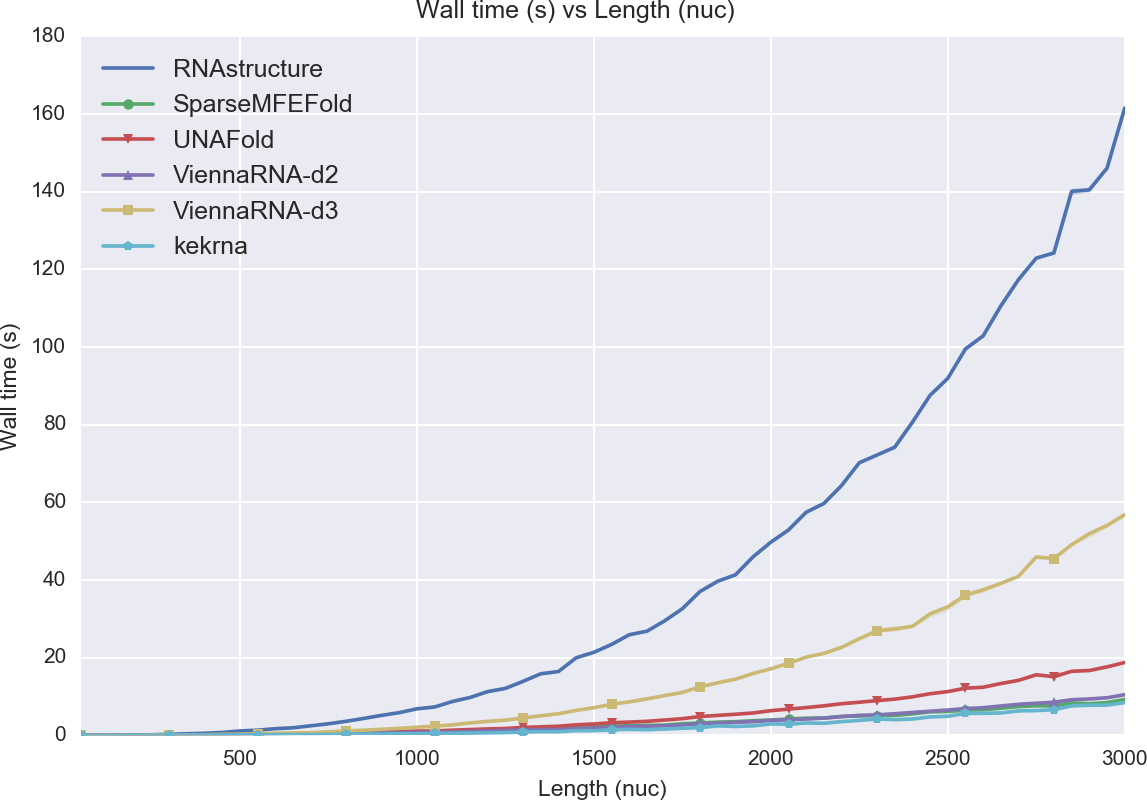
\includegraphics[width=0.9\textwidth]{res/random_real.png}
\caption{Random dataset---Wall time}
\label{fig:random_real}
\end{figure}

\begin{figure}[p]
\centering
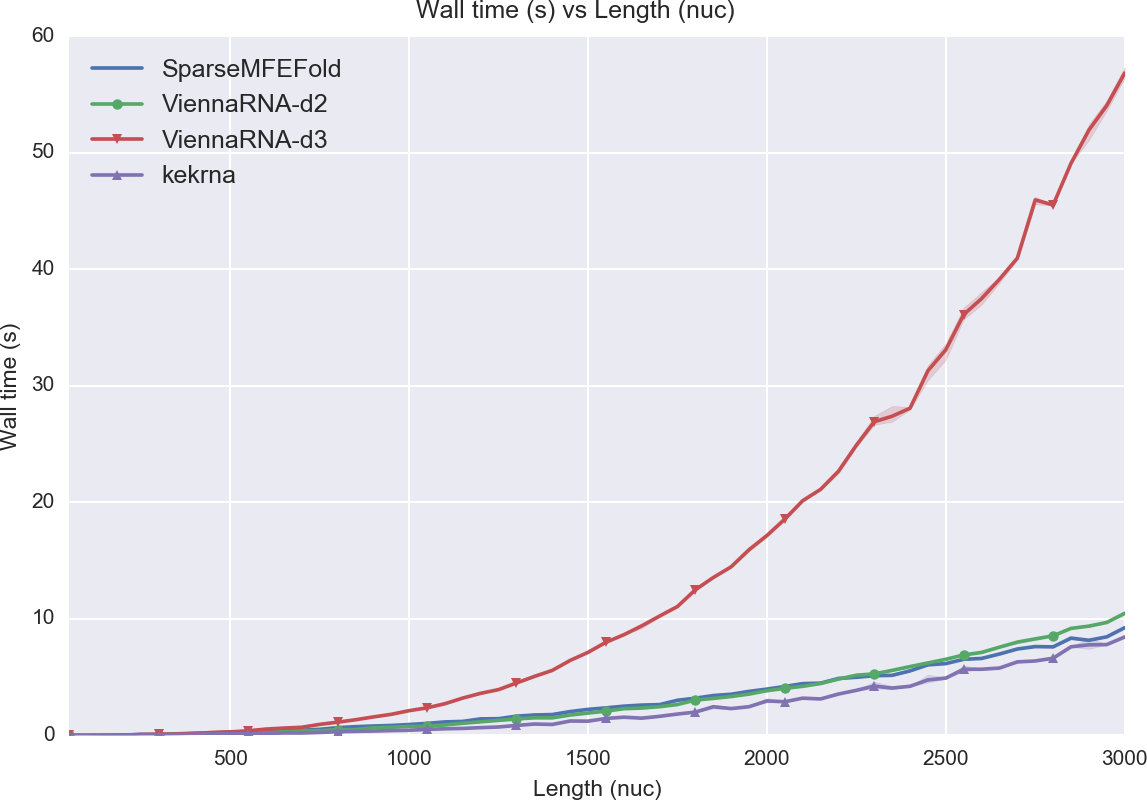
\includegraphics[width=0.9\textwidth]{res/random_fast_real.png}
\caption{Random dataset---Top three---Wall time}
\label{fig:random_fast_real}
\end{figure}

The runtimes of six configurations are displayed in \autoref{fig:random_real}, for each length of RNA in the random dataset. What we can see from this figure is that, in general, RNAstructure is by far the slowest, followed by ViennaRNA-d3 and UNAFold. Faster than that is ViennaRNA-d2, followed by SparseMFEFold and then kekrna. It is a bit hard to see the difference between the last three, so I have shown just those in \autoref{fig:random_fast_real}. Kekrna does the same amount of ``work" as RNAstructure and more than ViennaRNA-d3, since ViennaRNA-d3 does not handle certain types of coaxial stacks \cite{viennaBroken}. ViennaRNA-d2 assumes that every unpaired adjacent base dangles, and SparseMFEFold has the same behaviour as ViennaRNA with the d0 option, which does not consider any CTDs at all \cite{willSparseFolding}.

Suppose we have some polynomial $y = a_n x^n + a_{n-1}x^{n-1} ... a_0$. Taking the log of both sides, we have $\log(y) = \log(a_n x^n + a_{n-1}x^{n-1} ... a_0)$. As $x$ tends towards infinity, the highest order term in the polynomial will dominant, and we will have $y \approx a_n x^n$. Substituting this, we get $\log(y) = n \log(x) + \log(a_n)$. By plotting the results on a log-log scale graph and taking a linear regression, we can see how close each algorithm is to what it should be for a Zuker-Stiegler algorithm implementation: $O(N^3)$ \cite{zukerDp}. We can also estimate the constant factor overhead by computing the value of $a_n$.

\begin{figure}[p]
\centering
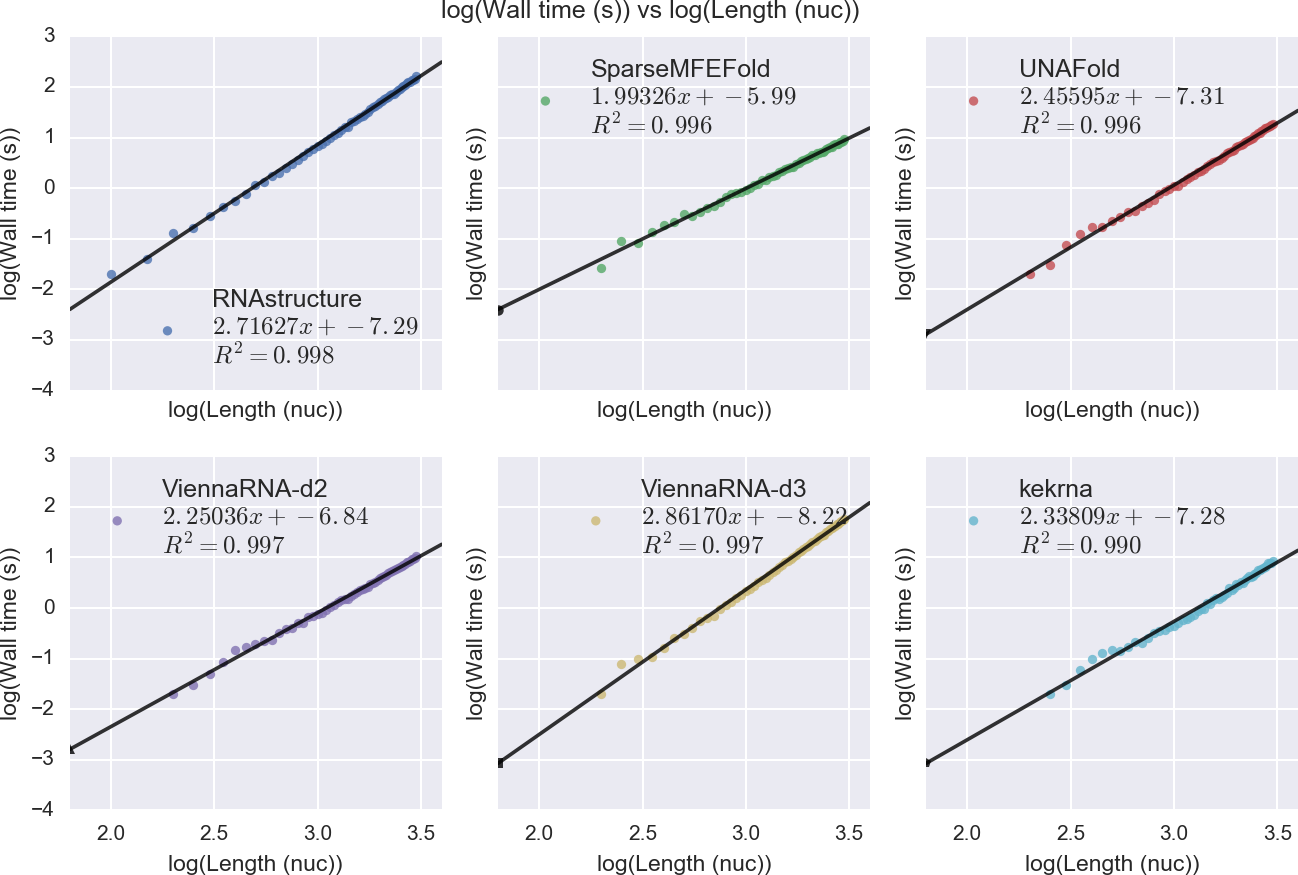
\includegraphics[width=0.9\textwidth]{res/random_real_loglog_scatter.png}
\caption{Random dataset---Wall time log-log scatter}
\label{fig:random_real_loglog_scatter}
\end{figure}

\begin{figure}[p]
\centering
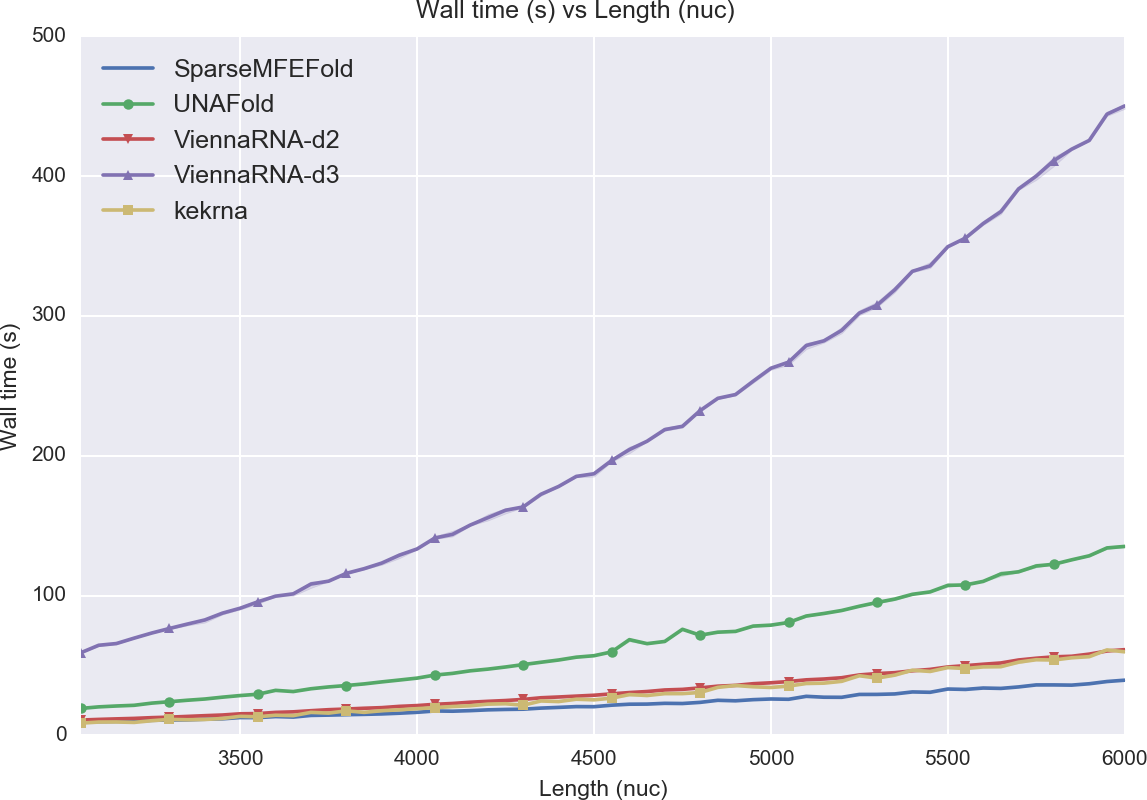
\includegraphics[width=0.9\textwidth]{res/random_large_real.png}
\caption{Large random dataset---Wall time}
\label{fig:random_large_real}
\end{figure}

In \autoref{fig:random_real_loglog_scatter}, the runtimes and lengths are plotted on a log-log scale, along with a line of best fit, its equation, and the $R^2$ value. The lines of best fit seem fairly well determined, so we can say that, empirically, the runtimes of these implementations grows with some polynomial. We can see from the slopes, for RNAs larger than three thousand nucleotides, SparseMFEFold and ViennaRNA-d2 are likely to run faster than kekrna.  \autoref{fig:random_large_real} goes from three thousand to six thousand nucleotides, and shows that for very large RNA, SparseMFEFold is faster, and ViennaRNA-d2 looks slightly faster at length six thousand. However, the Turner 2004 energy model does not work very well for RNAs much longer than one thousand nucleotides, so being faster in the below three thousand nucleotide area is arguably more important.  A summary of the empirical complexity results is in \autoref{table:random_complexity}. Note that these complexities change in the large random dataset, so should be taken with a large grain of salt.

\rowcolors{1}{white}{verylightgray}
\begin{table}
\begin{adjustbox}{center}
\begin{tabular}{ll}
Package & Approximate runtime  \\
kekrna & $O(N^{2.34})$ \\
RNAstructure & $O(N^{2.72})$ \\
RNAstructure-mod & $O(N^{2.75})$ \\
SparseMFEFold & $O(N^{1.99})$ \\
UNAFold & $O(N^{3.06})$ \\
ViennaRNA-d2 & $O(N^{2.25})$ \\
ViennaRNA-d3 & $O(N^{2.86})$ \\
\end{tabular}
\end{adjustbox}
\caption{Approximate time complexities for up to size 3000 RNAs}
\label{table:random_complexity}
\end{table}
\rowcolors{1}{white}{white}

In \autoref{fig:random_maxrss} we can see the memory usage, in terms of maximum resident set size. Overall, kekrna had the highest memory usage, followed by RNAstructure, UNAFold, ViennaRNA-d2, ViennaRNA-d3, and finally SparseMFEFold, which unsurprisingly had the least memory usage. Note that the two ViennaRNAs have almost exactly the same memory usage so they show up as one line. Overall, memory seems not as important, as all of the packages use a reasonable amount of memory for the size of RNA people would want to fold (on the order of thousands of nucleotides). \autoref{fig:random_large_maxrss_loglog_scatter} shows the log-log graph of memory usage for the large random dataset. The graph for the random dataset is quite noisy and not useful. Looking at the equations of the lines of best fit, we see that everything has about $O(N^2)$ memory usage, except for SparseMFEFold which has $O(N)$ memory usage. This is as expected.

\begin{figure}[p]
\centering
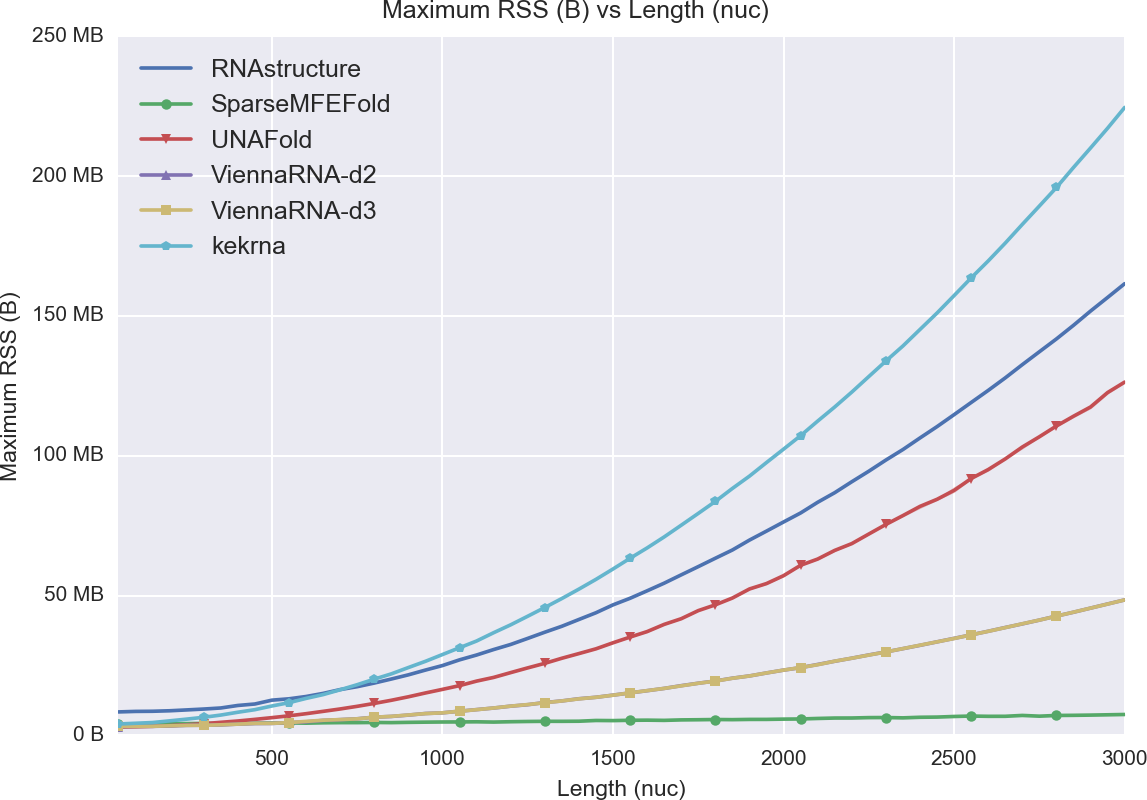
\includegraphics[width=0.9\textwidth]{res/random_maxrss.png}
\caption{Random dataset -- Maximum RSS}
\label{fig:random_maxrss}
\end{figure}

\begin{figure}[p]
\centering
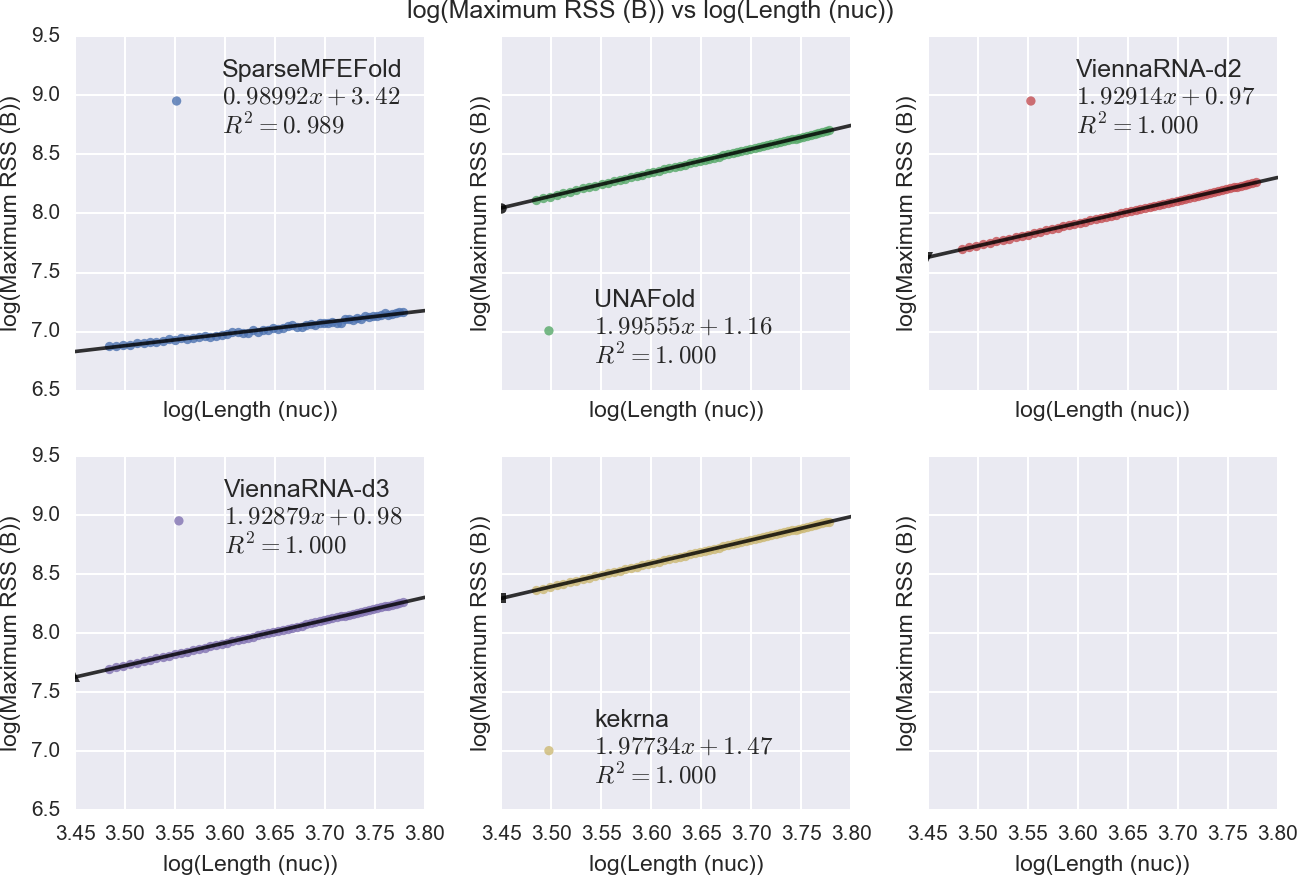
\includegraphics[width=0.9\textwidth]{res/random_large_maxrss_loglog_scatter.png}
\caption{Large random dataset---Maximum RSS log-log scatter}
\label{fig:random_large_maxrss_loglog_scatter}
\end{figure}

I conclude from these figures that kekrna is faster than every other package tested for RNAs up to length three thousand, despite fully implementing coaxial stacking. While it uses more memory, I think it is a reasonable amount. It is possible to halve kekrna's memory usage easily by changing the energy data type to \texttt{int16\_t} (like RNAstructure) from \texttt{int32\_t}, if this is an issue.

\subsection{Accuracy Results}

I was given permission to use the database of David Mathews et al., Archive II, of RNA structures \cite{mathewsPersonal}, which I used to test the accuracy of the programs, i.e. PPV, sensitivity, and F-score. This only contains secondary structures that have been verified with comparative sequence analysis, nuclear magnetic resonance, or X-ray crystallography---other secondary structures would be at least partly algorithmically computed with algorithms similar to those that I tested and would bias the results. I only looked at the domains of the RNA in Archive II, with duplicates (by primary and secondary structure together) removed, totalling 3459 secondary structures---the data describing which these were given to me by Ward \cite{wardPersonal}.

I was only looking at improving performance, rather than the accuracy. But, it is still interesting to take a look at the differences in accuracy between the programs. \autoref{table:archiveii} shows, most importantly, the mean F-score of each package. ViennaRNA-d2 has the highest F-score, but I believe they have optimised their parameters to get a higher F-score on the currently well-known set of RNA secondary structures. RNAstructure-mod, Ward's and my modified version of RNAstructure that corrects the bugs discussed in \autoref{chap:work}, has a higher F-score than RNAstructure. This suggests those bug fixes are significant. Looking at the distributions of F-score in \autoref{fig:archiveii_fscore}, it looks normal enough to perform a paired t-test. I checked the kurtosis and skew values for the F-scores for each package, and they were all less than one in absolute value. \autoref{table:archiveii_ttest} has the results of the t-test, with the $t$-values in the bottom half, and the $p$-values in the upper half. The null hypothesis was that the mean F-score of the RNA package in row $i$ is equal to the mean F-score of the RNA package in column $j$, where $i > j$ (looking at only the bottom half of the triangle). For example, looking at the row ``RNAstructure" and the column ``UNAFold" gives a $p$-value of approximately zero, showing that the probability that these results occurred by chance given the null hypothesis, i.e. that UNAFold's F-score mean is the same to that of RNAstructure's, is approximately zero.

It looks like RNAstructure-mod is more accurate according to the F-score measure ($p=0.005$), meaning that these bugs ought to be fixed in the main RNAstructure distribution. Kekrna is not as accurate as RNAstructure ($p=0.014$), which is interesting, as it always produced the same MFE as RNAstructure-mod. I think this is just a quirk of the ordering of the recurrences. If it is an issue, you could permute the order of the cases in \texttt{src/fold/traceback.cpp} to get kekrna to produce the same MFE structure as RNAstructure, or even use a genetic algorithm to optimise them for F-score. It would be a permutation based genetic algorithm using the order of the cases in \texttt{src/fold/traceback.cpp}. The fitness function would be the F-score on Archive II.

\begin{figure}[h]
\centering
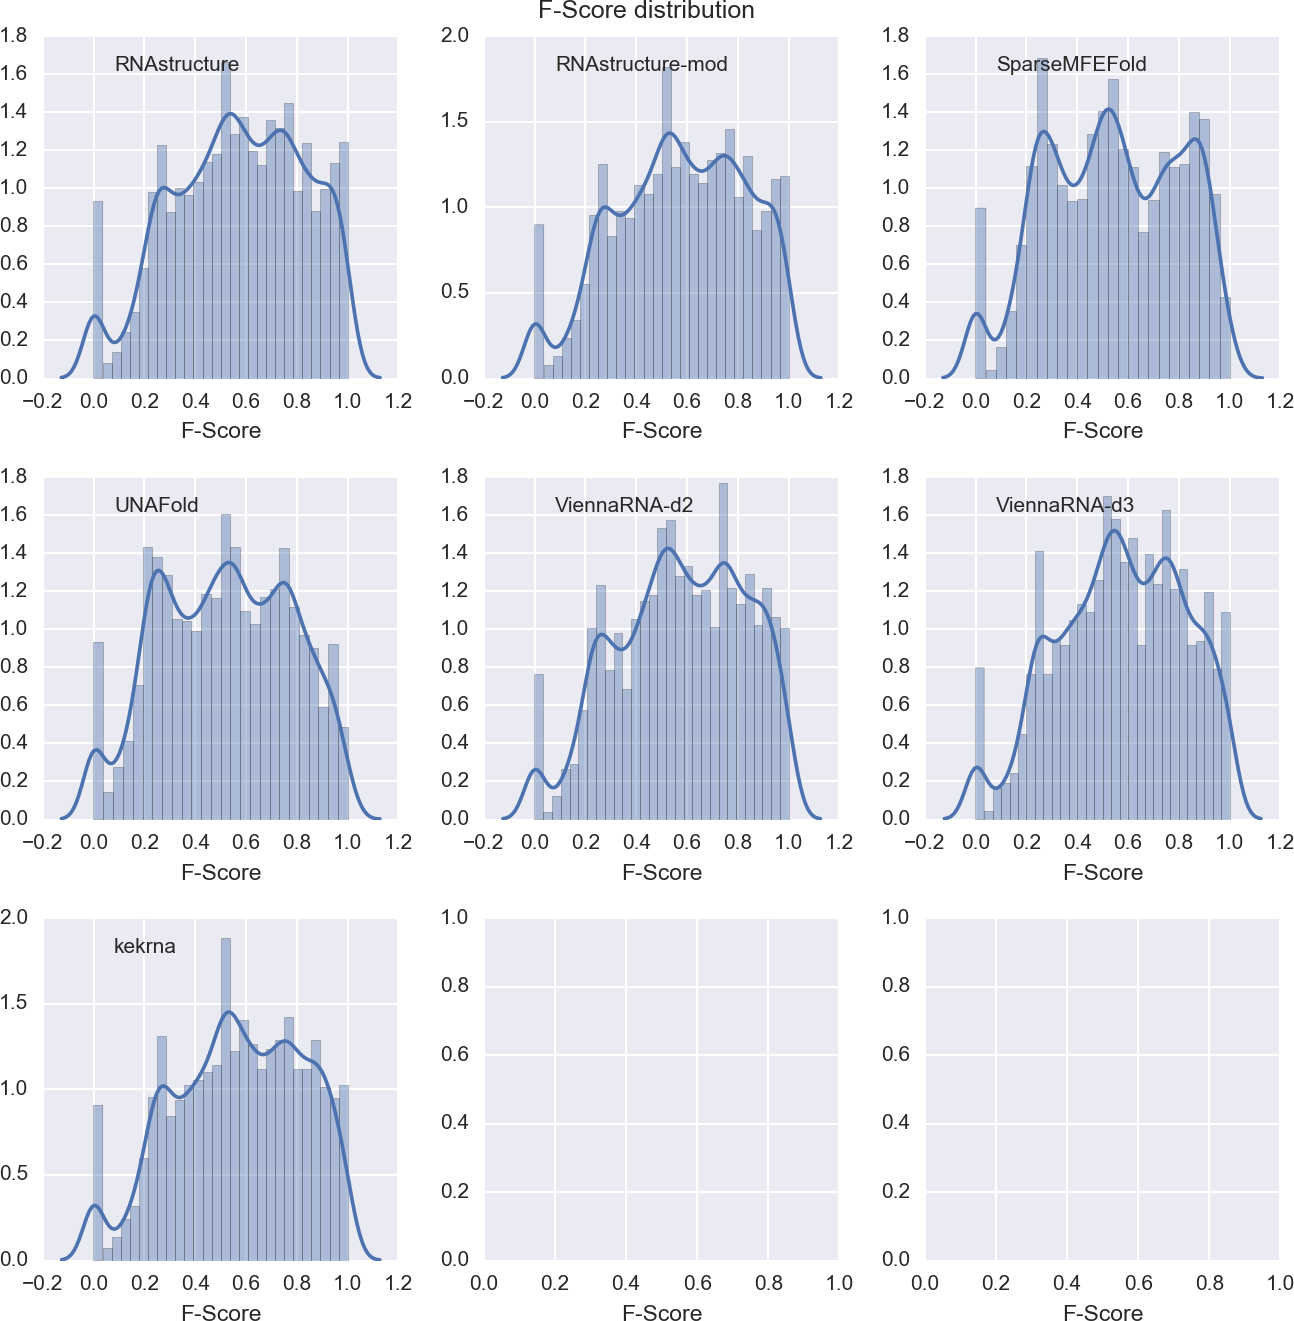
\includegraphics[width=0.8\textwidth]{res/archiveii_domains_fscore.png}
\caption{Archive II domains---F-Score distribution}
\label{fig:archiveii_fscore}
\end{figure}

\begin{landscape}
\rowcolors{1}{white}{verylightgray}
\begin{table}
\begin{adjustbox}{center}
\begin{tabular}{lllllll}
Package & F-Score mean & F-Score SD & PPV mean & PPV SD & Sensitivity mean & Sensitivity SD \\
RNAstructure & 0.57058 & 0.25539 & 0.54759 & 0.25587 & 0.60037 & 0.25714 \\
RNAstructure-mod & 0.57229 & 0.25362 & 0.54938 & 0.25395 & 0.60201 & 0.25557 \\
SparseMFEFold & 0.53954 & 0.25790 & 0.51550 & 0.25398 & 0.57055 & 0.26512 \\
UNAFold & 0.51776 & 0.25432 & 0.49319 & 0.24987 & 0.54984 & 0.26242 \\
ViennaRNA-d2 & 0.57644 & 0.25027 & 0.54934 & 0.24795 & 0.61115 & 0.25522 \\
ViennaRNA-d3 & 0.57216 & 0.24630 & 0.54591 & 0.24487 & 0.60588 & 0.25031 \\
kekrna & 0.56897 & 0.25234 & 0.54589 & 0.25245 & 0.59887 & 0.25455 \\
\end{tabular}
\end{adjustbox}
\caption{Archive II domains---Accuracy results}
\label{table:archiveii}
\end{table}
\rowcolors{1}{white}{white}

\rowcolors{1}{white}{verylightgray}
\begin{table}
\begin{adjustbox}{center}
\begin{tabular}{llllllll}
Package & RNAstructure & RNAstructure-mod & SparseMFEFold & UNAFold & ViennaRNA-d2 & ViennaRNA-d3 & kekrna \\
RNAstructure & --- & 0.005 & 0.000 & 0.000 & 0.000 & 0.265 & 0.014 \\
RNAstructure-mod & 2.816 & --- & 0.000 & 0.000 & 0.003 & 0.926 & 0.000 \\
SparseMFEFold & -15.073 & -16.138 & --- & 0.000 & 0.000 & 0.000 & 0.000 \\
UNAFold & -25.186 & -25.936 & -10.046 & --- & 0.000 & 0.000 & 0.000 \\
ViennaRNA-d2 & 4.182 & 2.998 & 19.368 & 28.591 & --- & 0.001 & 0.000 \\
ViennaRNA-d3 & 1.115 & -0.093 & 15.360 & 25.377 & -3.475 & --- & 0.022 \\
kekrna & -2.449 & -12.155 & 14.538 & 24.522 & -5.415 & -2.290 & --- \\
\end{tabular}
\end{adjustbox}
\caption{Archive II domains---Paired t-test results}
\label{table:archiveii_ttest}
\end{table}
\rowcolors{1}{white}{white}
\end{landscape}

\section{Suboptimal Folding Tests}
It was much harder to evaluate the performance of the packages for suboptimal folding. I did not attempt to evaluate the accuracy, other than showing that RNAstructure's implementation was buggy, and that ViennaRNA's did not produce structures with different CTD configurations---see \autoref{chap:work}. I tested each program by having it output its generated structures to a file, redirecting from \texttt{stdout} if it did not have an option to write to a file directly. I then counted the number of lines using \texttt{wc -l}, and subtracted some number (which varies per program) to get the correct number of structures produced. I had trouble testing kekrna's performance for two reasons. The first was that kekrna regularly generates structure output at over 500 MiB/s, which is more than the approximately 450 MiB/s mSATA SSD in my laptop could handle. Secondly, in the five limit timespan, kekrna would fill up my entire SSD with structures and stop. I did not have this problem with any of the other packages.

I ran each program on the random dataset for energy deltas of 0.1, 0.2, 0.3, 0.4, 0.5, 0.6, 1.0, 1.1, 1.2, and 1.3 
kcal/mol, using the command-line arguments shown in \autoref{table:suboptimal_run_commands}. SparseMFEFold only does MFE folding, and UNAFold appears to only support Zuker-type suboptimal folding, which does not generate all suboptimal structures \cite{zukerSuboptimal}. So I left them out. Schroeder Lab's RNAsubopt++ is new in this section. It can optionally be run using OpenMPI, which parallelises it. I set it to use four processes, because I found that it was not faster when I set it to use eight processes on my 4-core hyperthreaded processor. It also has an option to use some updated parameters closer to the Turner 2004 model, which I enabled. It does not support coaxial stacking at all, however.

\rowcolors{1}{white}{verylightgray}
\begin{table}
\begin{adjustbox}{center}
\begin{tabular}{lp{10cm}}
RNAstructure &\texttt{DATAPATH=<datapath> AllSub -a <delta> <in> <out>} \\
ViennaRNA-d2 &\texttt{echo <in> | RNAsubopt -d2 -e <delta> > <out>} \\
ViennaRNA-d3 &\texttt{echo <in> | RNAsubopt -d3 -e <delta> > <out>} \\
ViennaRNA-d2-sorted &\texttt{echo <in> | RNAsubopt -d2 --sorted -e <delta> > <out>} \\
ViennaRNA-d3-sorted &\texttt{echo <in> | RNAsubopt -d3 --sorted -e <delta> > <out>} \\
SJSViennaMPI &\texttt{mpirun -n 4 RNAsubopt -P 2004.par -d2 -e <delta> -input <in>} \\
SJSViennaMPI-sorted &\texttt{mpirun -n 4 RNAsubopt -P 2004.par -d2 --sorted -e <delta> -input <in>} \\
kekrna & \texttt{subopt -delta <delta> <in> > <out>} \\
kekrna-sorted & \texttt{subopt -sorted -delta <delta> <in> > <out>} \\
\end{tabular}
\end{adjustbox}
\caption{Suboptimal folding run commands}
\label{table:suboptimal_run_commands}
\end{table}
\rowcolors{1}{white}{white}

\begin{figure}[p]
\centering
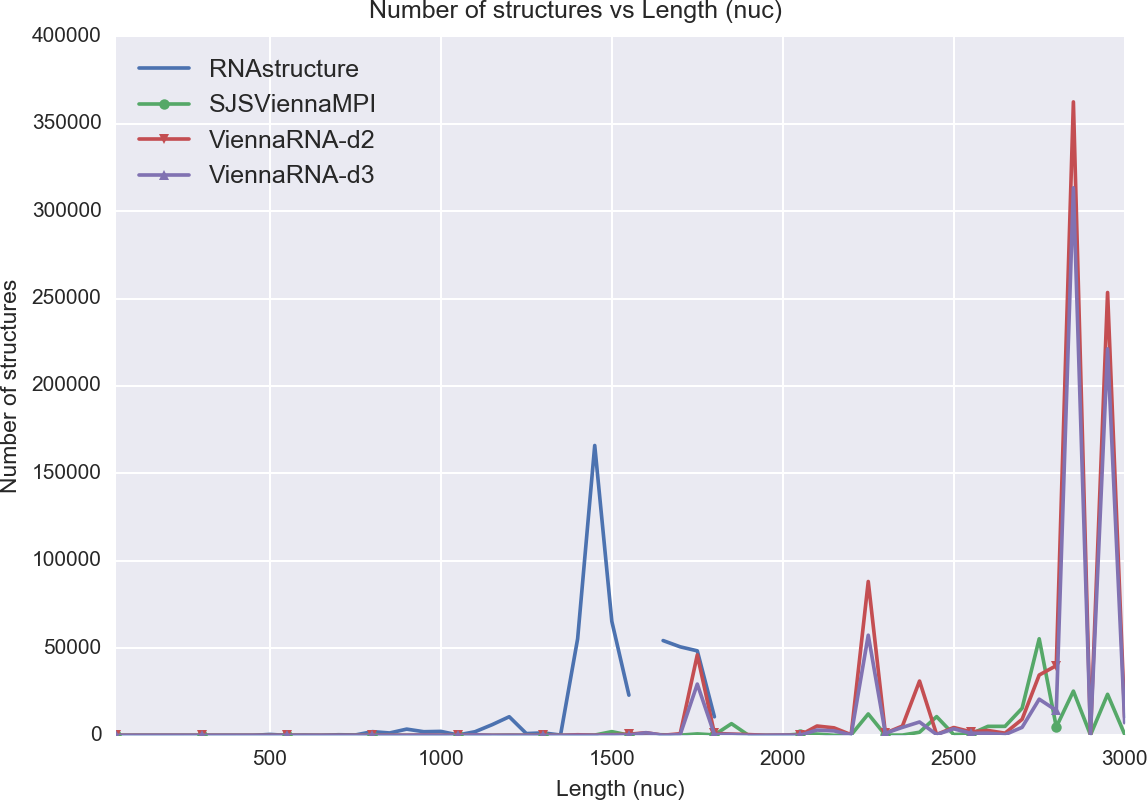
\includegraphics[width=0.9\textwidth]{res/subopt_1_numstruc.png}
\caption{Random dataset---Delta 1---Number of structures}
\label{fig:subopt_1_numstruc}
\end{figure}

\begin{figure}[p]
\centering
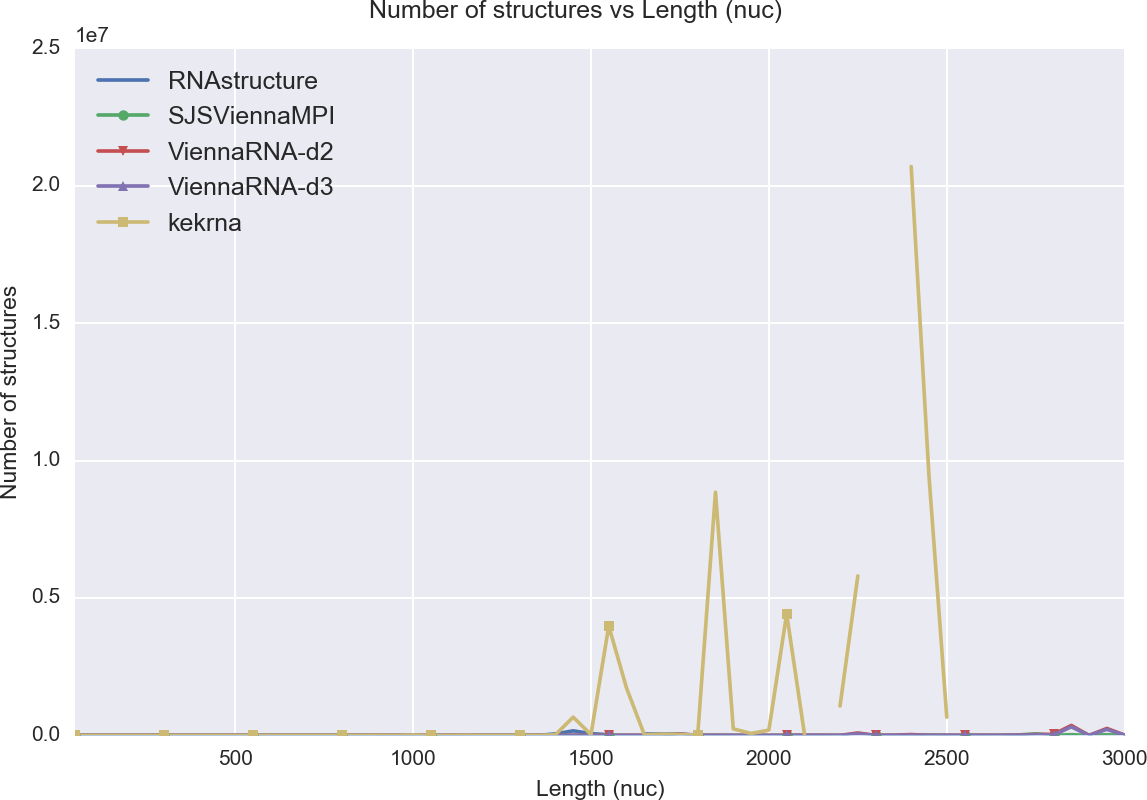
\includegraphics[width=0.9\textwidth]{res/subopt_1_numstruc_with_kekrna.png}
\caption{Random dataset---Delta 1---Number of structures with kekrna}
\label{fig:subopt_1_numstruc_with_kekrna}
\end{figure}

Looking at \autoref{fig:subopt_1_numstruc}, we can see that the number of structures produced by each program is highly variable---the sorted versions are omitted since they should output the same number of structures. This, and the bugs in existing programs makes it hard to compare the run-times between them. Adding kekrna into the mix shows that the other programs are missing huge numbers of structures, as you can see in \autoref{fig:subopt_1_numstruc_with_kekrna}. These graphs also have breaks in them, making them hard to read. Instead, I think it is better to look at the distribution of number of structures generated per second. This is shown in \autoref{fig:subopt_distribution_numstruc} and \autoref{table:structures_per_second}. RNAstructure has a maximum of around 4500 structures per second, compared to the 30000 to 40000 of the other packages. Kekrna, however, has a maximum of 600000, and a much higher mean and median.

\begin{figure}[h]
\centering
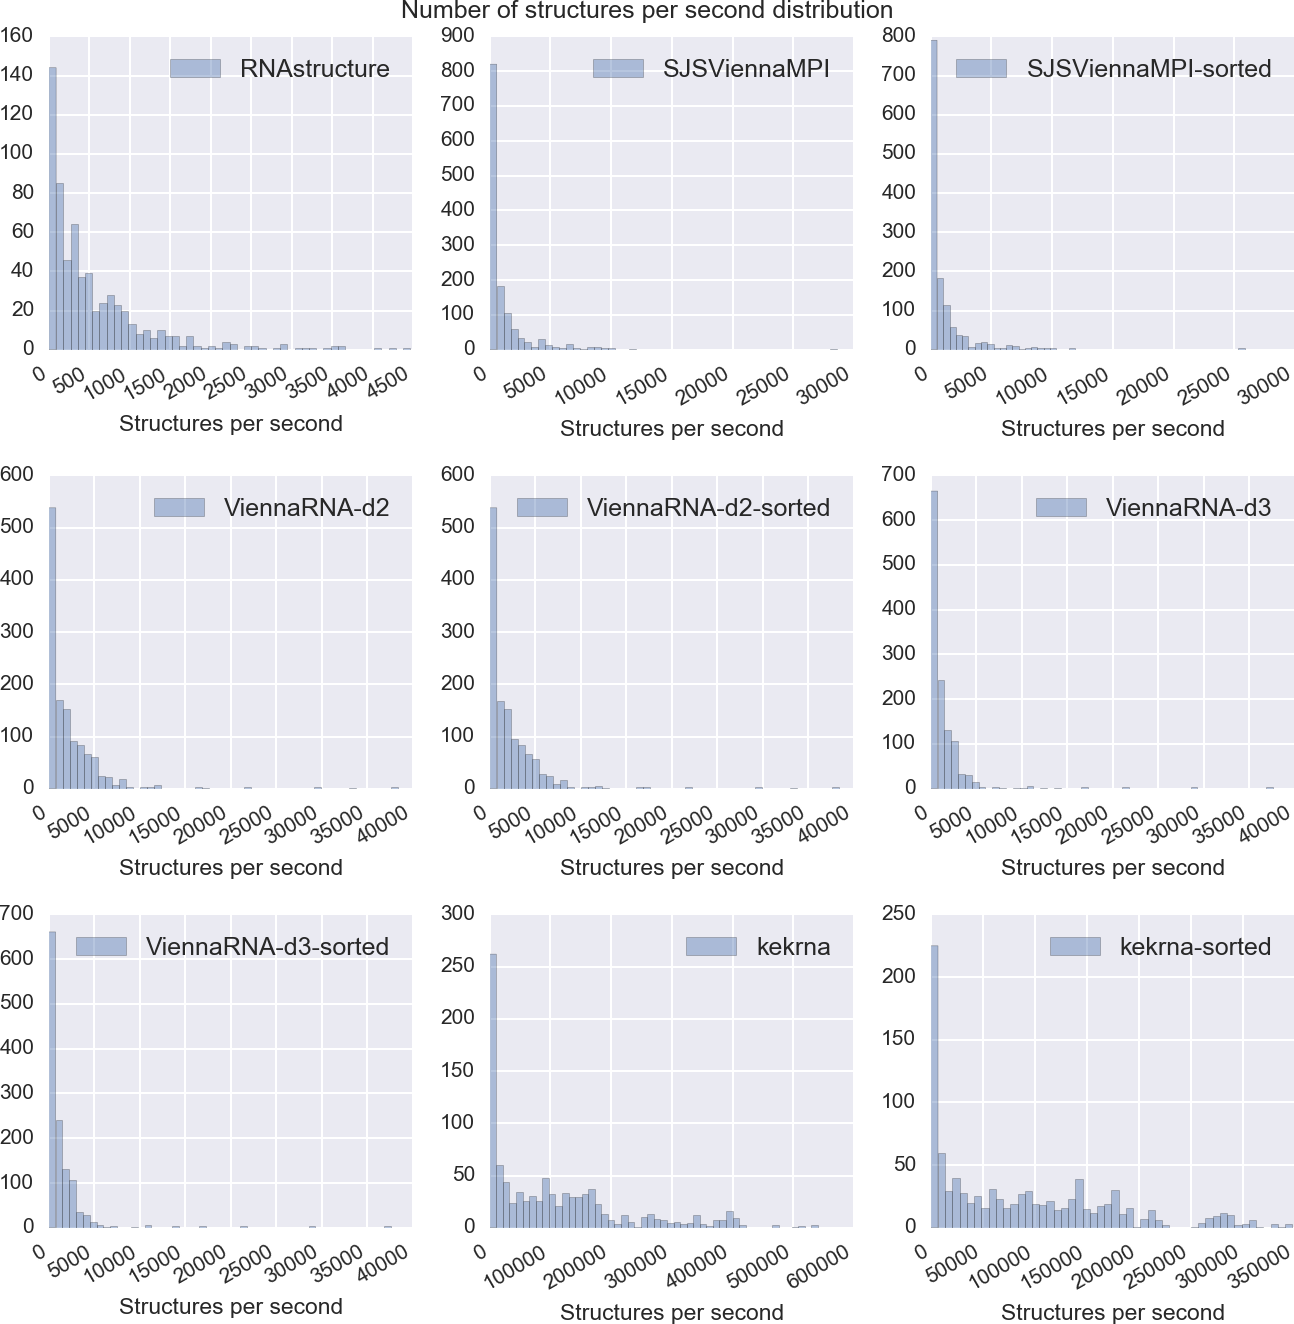
\includegraphics[width=0.8\textwidth]{res/subopt_distribution_numstruc.png}
\caption{Distribution of number of structures per second}
\label{fig:subopt_distribution_numstruc}
\end{figure}

\rowcolors{1}{white}{verylightgray}
\begin{table}
\begin{adjustbox}{center}
\begin{tabular}{llll}
Package & Structures/s mean & Structures/s SD & Structures/s median \\
RNAstructure & 556.2 & 683.7 & 303.7 \\
SJSViennaMPI & 1095.1 & 2223.9 & 312.1 \\
SJSViennaMPI-sorted & 1087.6 & 2134.4 & 314.8 \\
ViennaRNA-d2 & 2235.0 & 3613.2 & 1230.8 \\
ViennaRNA-d2-sorted & 2224.7 & 3525.5 & 1246.8 \\
ViennaRNA-d3 & 1384.4 & 2972.4 & 606.0 \\
ViennaRNA-d3-sorted & 1402.4 & 2990.5 & 600.0 \\
kekrna & 105788.8 & 114587.2 & 76280.6 \\
kekrna-sorted & 85213.4 & 84008.8 & 63460.0 \\
\end{tabular}
\end{adjustbox}
\caption{Structures per second}
\label{table:structures_per_second}
\end{table}
\rowcolors{1}{white}{white}

I also wanted to compare kekrna to the currently fastest package, ViennaRNA. Since ViennaRNA generates far fewer structures than kekrna, I tried using kekrna's max-delta functionality to see how long it would take to generate the same number of structures as ViennaRNA. This is potentially not a fair comparison because to get the same number of structures, kekrna might have to explore less of the folding landscape---I am not sure because it depends on how ViennaRNA is implemented. The results are in \autoref{fig:subopt_max_real}, and show that kekrna is much faster for generating the same number of structures.

\autoref{fig:subopt_1_maxrss_sorted_comparison} shows a comparison of memory between kekrna-sorted, ViennaRNA-d2, and ViennaRNA-d2-sorted. When ViennaRNA is given the \texttt{--sorted} option, it takes much more memory. This is likely because it needs to store all structures in memory before sorting them. Kekrna instead uses iterated depth-first searches to avoid storing everything in memory for sorted output, and this is shown in the graph. 


\begin{figure}[p]
\centering
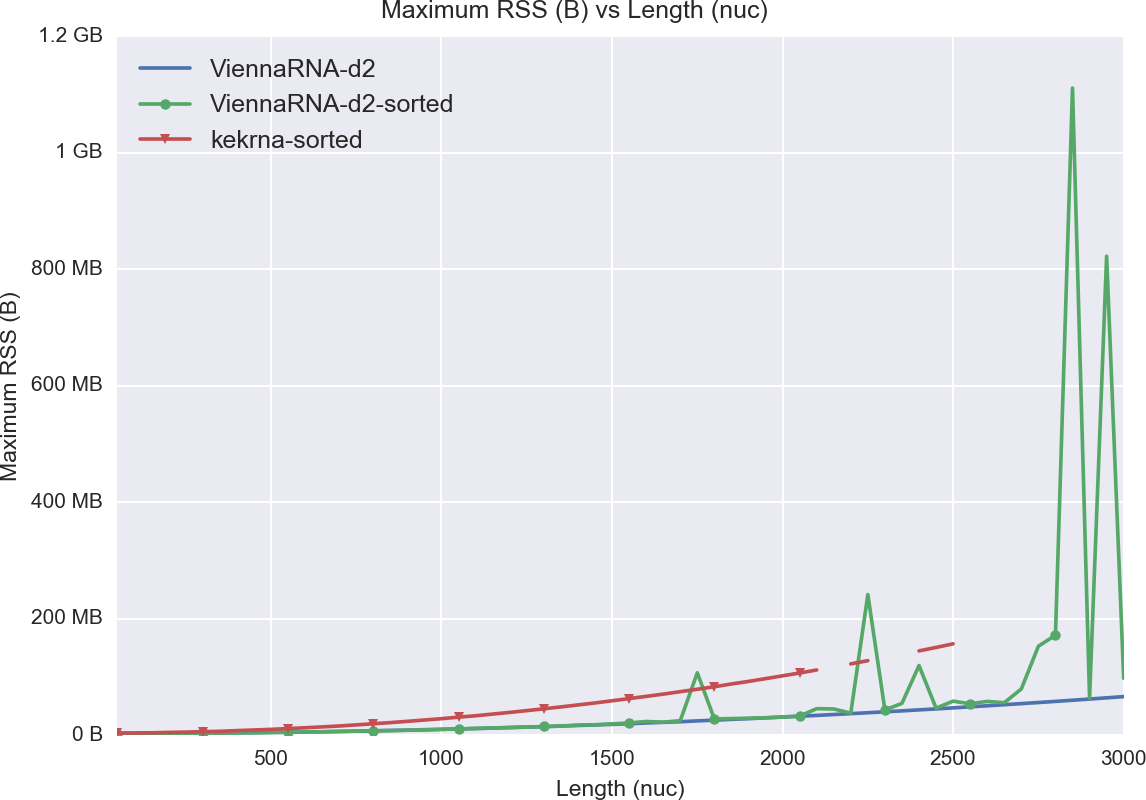
\includegraphics[width=0.9\textwidth]{res/subopt_1_maxrss_sorted_comparison.png}
\caption{Random dataset---Delta 1---sorted comparison---Maximum RSS}
\label{fig:subopt_1_maxrss_sorted_comparison}
\end{figure}

\begin{figure}[p]
\centering
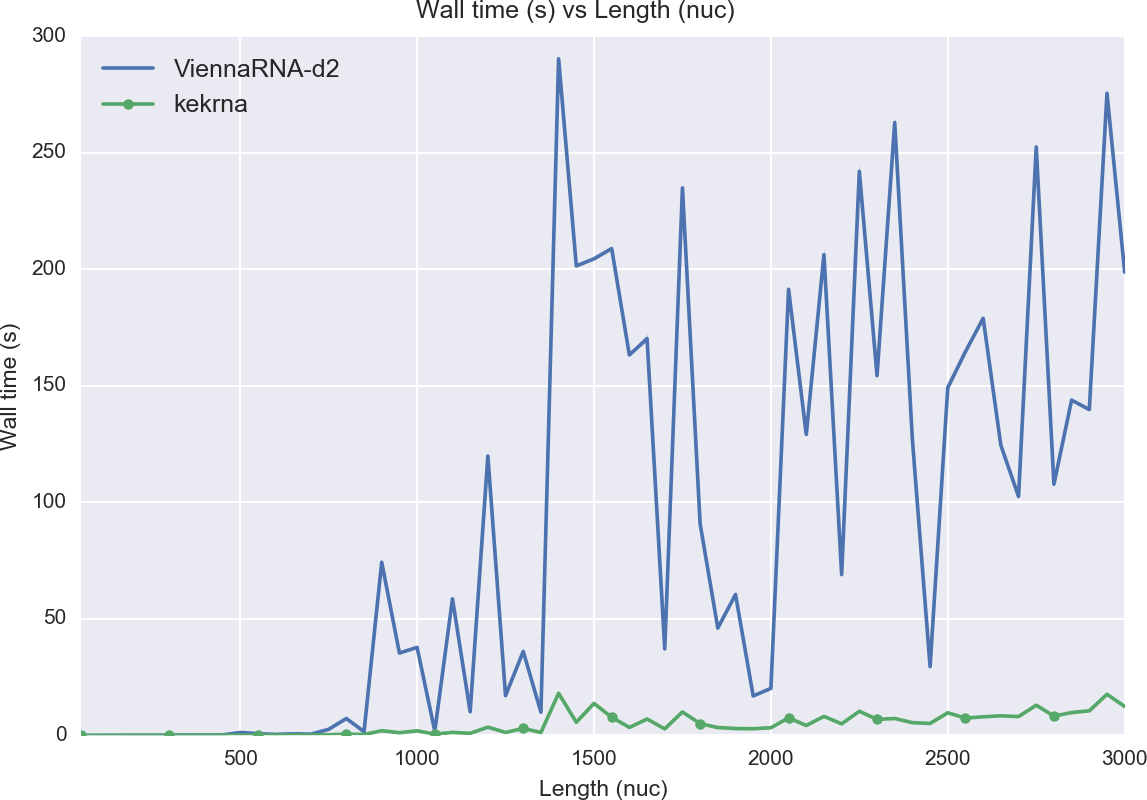
\includegraphics[width=0.9\textwidth]{res/subopt_max_real.png}
\caption{Random dataset---Matching ViennaRNA's structure counts---Wall time}
\label{fig:subopt_max_real}
\end{figure}

Overall, while it is harder to compare between suboptimal folding implementations, I think kekrna is faster than the other packages by a significant amount.

\chapter{Conclusion}
\section{Future Work}
It might be useful to extend kekrna to be configurable with a larger set of the energy model parameters, or implement any other common features it might be missing. 

A genetic algorithm to evolve a trace-back ordering to maximise the F-score on Archive II, and an analysis of what the more optimal orderings imply could be good. 

The partition function implementation in kekrna is relatively un-optimised, and, while you can compile it with MPFR \cite{mpfr} for arbitrary precision floats, finding a solution to the precision issues that seem to be common to all partition function implementations could be a good project.

\section{Conclusion}
My goal was to extend sparse folding to the Zuker-Stiegler algorithm with coaxial stacking. I did that with the invention of the kek manoeuvre, as well as inventing a new type of sparse optimisation for the algorithm of Wuchty et al. These improvements were not just theoretical---my other main contribution is kekrna, a fast folding package. In empirical tests, kekrna is much faster than other popular RNA folding packages, in both MFE folding and suboptimal folding. It is also truer to the energy model. In writing kekrna, I discovered several bugs in RNAstructure, which I reported to David Mathews, and several omissions in ViennaRNA. I think this, and having a separate, well-tested implementation existing for the energy model, MFE folding, and suboptimal folding is useful to the RNA folding community.

\begin{appendices}
\chapter{Original Honours Proposal}

\section*{Background}
RNA (ribonucleic acid) is a bit like DNA, although it only has one strand. It is composed of a backbone made of sugars, and 'bases' attached to those sugars. The bases in RNA are guanine, uracil, adenine, and cytosine, which we write down like this when describing RNA: "GUAC." Just like in DNA, these bases have other bases that they like to bond to. In RNA, these bonds happen between guanine and uracil (GU), guanine and cytosine (GC), and adenine and uracil (AU). Because RNA is single-stranded, when the bases bond, they can bond to the RNA itself. This makes the RNA "fold," and assume a shape, which we call its secondary structure. Knowing the secondary structure of RNA is useful for biologists to predict how the RNA will act.\cite{connRnaBackground}

One of the major approaches to predicting how an RNA will fold is free energy minimisation. Free energy is, loosely, a measure of how much energy is available to do work in a system \cite{perrotThermodynamics}. The thermodynamic hypothesis \cite{anfinsenThermodynamicHypothesis} tells us to assume the structure RNA will assume in vivo (in real life conditions) will be one with minimum free energy---this is also supported by evidence \cite{tinocoHowRnaFolds}. To compute the free energy of a folding, we need a model telling us how. One of the current popular models is the Nearest Neighbour model, the parameters of which were first compiled by Turner \etal in 1999\cite{t99}, updated in 2004\cite{t04}, and then used to create the Nearest Neighbour Database (NNDB) in 2009 \cite{tNndb}. By using this model as an approximation, we can try to predict the secondary structure of RNA by finding the structure that minimises the free energy.

\subsection*{The Zuker-Stiegler algorithm}
The Zuker-Stiegler algorithm is an important dynamic programming algorithm in computational RNA folding. Given an energy model, it will compute the secondary structure with the minimum free energy in $O(N^3$) time using $O(N^2)$ memory\cite{zukerDp}. There are several popular implementations of this algorithm: ViennaRNA's RNAfold\cite{viennarna}, RNAstructure\cite{rnastructure}, and mfold\cite{mfold}.

\section*{Aim and the Problem}
My goal is to write an optimised implementation of the Zuker-Stiegler algorithm, with better performance than all existing implementations. This will hopefully allow biologists to fold larger RNA. The aforementioned RNAfold is the fastest implementation I've seen so far, so for now I'll take it as the one to beat.

\subsection*{Algorithmic Improvements}
I hope to apply both generic dynamic programming optimisations and ones specific to the Zuker-Stiegler algorithm. Eppstein \etal suggest several general optimisations to dynamic programming algorithms based on properties of the function being optimised \cite{eppsteinSpeedingUpDp}. They further suggest that the Zuker-Stiegler algorithm may be optimised to $O(N^2\log{N}\log{\log{N}})$. Also, F. Yao has proven that in some cases the \emph{quadrangle inequality} may be exploited to reduce complexity by a linear factor \cite{yaoSpeedingUpDp}. There seem to be a lot of general techniques I could try to apply here, so I will systematically go through them and evaluate which improve performance in practice.

\subsection*{Implementation Improvements}
Modern hardware performs many optimisations by itself to try to improve speed, such as: pre-fetching, instruction reordering, branch prediction, and multi-level caching \cite{drepperMemory}. Programs running on the CPU can be very sensitive to memory access orderings and similar; this is even more apparent on the GPU. I would like to try to improve the Zuker-Stiegler algorithm's implementation by concentrating on these micro-optimisations---even a small performance improvement inside a doubly nested loop can give a large overall performance benefit.

I would also like to experiment with a GPGPU implementation of the algorithm if I have time. This has been done before by Guoqing Lei \etal \cite{leiGpu} and Guillaume Rizk \etal \cite{rizkGpu}, but not using an up to date version of the Zuker-Stiegler algorithm. The original algorithm was $O(N^4)$, which was later optimised to $O(N^3)$ by limiting a loop to at most 30 iterations \cite{lyngsoOptimisation}. Later, Lyngso \etal optimised this to $O(N^3)$ without this limitation \cite{lyngsoPseudoknot}. 

\section*{Method and Plan}
I will begin by reading papers detailing the energy model, and then implement the Zuker-Stiegler algorithm myself. This will give me a good understanding of how the algorithm works in its entirety, which is useful for applying optimisations based specifically on the shape of the energy model, e.g. convexity. After that, I will read about optimisations from existing papers, implement them, and then examine their effect on the runtime. If I have time, I will consider a GPGPU implementation and try to come up with my own optimisations.

\end{appendices}

\bibliographystyle{IEEEtran}
\bibliography{IEEEabrv,honours}


\end{document}
